%\noindent {\bf Chapter editors:}~Xabier Cid Vidal, Heather Russell, Albert de Roeck, Jared Evans, David Curtin, Jose Zurita\\
%\text{ \; }\\
%\noindent {\bf Contributors:}~Juliette Alimena, Alberto Escalante del Valle, Philippe Mermod, Antonio Policchio, Brian Shuve\\
%\text{ \; }\\

%\noindent The goal of this chapter is to assess the capabilities of the existing long-lived particle searches at ATLAS, CMS and LHCb, and to identify any potential gaps in coverage.

\noindent A critical component of any discussion of long-lived particle searches at the LHC is the comprehensive review of the existing searches from ATLAS, CMS, and LHCb, and an assessment of their coverage and any gaps therein. This is an inherently challenging task, given the varied and atypical objects often defined and utilized in LLP analyses and the differences among the experiments. As such, the following discussion assumes little-to-no background on LLP search strategies and includes a high level of detail regarding the current analyses. The focus of the discussion is on the existing studies, while acknowledging that the landscape for new physics models and LLP signatures can be broader than the ones described here.

Backgrounds to most of these studies are typically small, as most LLP signatures are not naturally mimicked by any irreducible SM processeses. Backgrounds for LLP searches typically include peripheral or machine effects, those rarely important for searches for prompt physics, including cosmic muons, beam halo, detector noise, and cavern backgrounds. Such backgrounds are discussed in detail in Chapter~\ref{sec:backgrounds}. As rare as these backgrounds typically are, their rates are not completely negligible, and particular, model-dependent selection requirements (based on, for instance, the LLP mass range or specific decay modes) must be made to reduce backgrounds as much as possible and, in some cases, make the searches ``background-free''. Additionally, many default object reconstruction algorithms are not designed to detect particles originating from decays of LLPs, and so dedicated reconstruction of tracks, jets, leptons, or other objects may be required for LLP searches. Taken altogether, these factors make LLP searches very different from searches for prompt objects, and the following discussion additionally aims to collate and summarize the current techniques for LLP reconstruction at the LHC.

A particular challenge for many LLP signatures is the trigger. With the exception of certain dedicated ATLAS triggers in the calorimeters or muon spectrometer, there are no Level-1 (L1) triggers that directly exploit the displaced nature of LLP decays, and L1 trigger thresholds must be surpassed by standard objects (such as leptons or high-energy jets) for the event to be recorded. Throughout this chapter, we highlight the role and limitations of the trigger(s) employed in current searches, and the design of customized LLP triggers is to be encouraged to probe new and otherwise inaccessible regions of parameter space.

A detailed review of all existing searches is presented in Sections~\ref{subsec:djets} through \ref{subsec:funnytracks}. This survey of the current experimental coverage aims to highlight the highest-priority searches still yet to be performed, which we summarize in Section~\ref{sec:covgaps}. In all cases, we focus on the latest version of each analysis. Notably we will typically present searches based on data taken at a center-of-mass energy $\sqrt{s}=13$~TeV, and discuss searches using Run-1 data only when the newer version is not yet available, or when there are conceptual differences between two versions of the same analysis.

%{\bf BS:~Should we add a section where we have a few sentences about each of the searches that come out this summer?}

%{\bf \textcolor{red}{JB:~Agreed; it's a necessary addition.} }

Because long-lived particles travel macroscopic distances in the detectors, many of the search strategies rely on the identification of displaced objects, namely SM particles (charged leptons, photons, hadrons, jets) that are produced at a location away from the primary vertex (PV) where the hard $pp$ collision takes place. The secondary vertex at which the decay of the LLP occurs is referred to as a displaced vertex (DV). As far as possible, our classification of searches is linked to the parton-level objects produced in LLP decays, which allows a relatively straightforward linkage to LLP models (as well as simplified models; see Chapter~\ref{sec:simplifiedmodel}). Borrowing the terminology from prompt searches, we  consider the following categories for the analogous displaced objects produced in LLP decays: all-hadronic (jets), leptonic, semi-leptonic, and photonic. However, we caution the reader that these ``jets'' or ``photons'' may not be of the standard type, and so other objects may pass the selections of these analyses. The remaining searches  fall in the ``other long-lived exotics'' category, mostly consisting of non-standard tracks (disappearing tracks,  heavy stable charged particles, quirks, etc), but also including some trackless signals, such as stopped particles and Strongly Interacting Massive Particles (SIMPs). These categories are not to be interpreted as exclusive; many models and searches could fit into several categories.

\section{All-hadronic decays}
\label{subsec:djets}

ATLAS has several searches for displaced decays with hadronic objects, including searches for two objects decaying in the hadronic calorimeter (HCAL)~\cite{ATLAS-CONF-2016-103,CalRatio8TeV}; decays within the muon system (MS) or inner detector (ID)~\cite{Aad:2015uaa}; ID decays in association with large \met~\cite{Aaboud:2017iio}; and ID decays in association with large \met, jets, or leptons~\cite{Aad:2015rba}.  CMS has an inclusive search for displaced jets using 13 (8) TeV data~\cite{Sirunyan:2017jdo} (\cite{CMS:2014wda}). Moreover, the CMS displaced jets searches are relatively inclusive and so also cover LLPs with semi-leptonic decays despite having no specific lepton requirements. LHCb has searches for both one~\cite{Aaij:2017mic} and two~\cite{Aaij:2016isa} all-hadronic DVs in their detector. Here we restrict ourselves to summarize the hadronic channels, while those studies including leptons~\cite{Aad:2015rba,Sirunyan:2017jdo} will be revisited in Sections~\ref{subsec:dleptons} and \ref{subsec:dsemilep} for the fully-leptonic and semi-leptonic cases, respectively.

\subsection{ATLAS Searches}

The reconstruction of displaced tracks in the ATLAS ID~\cite{ATL-PHYS-PUB-2017-014} follows a two-step procedure. In the first iteration, the default track identification algorithm is applied, which uses hits in the pixel system, Semiconductor Tracker (SCT), and Transition Radiation Tracker (TRT) to reconstruct tracks with a small impact parameter.  The hits not associated to a track during the first pass are used in a second run of the track finder, with loose requirements on the transverse and longitudinal impact parameters ($d_{0}$ and $z_{0}$) and the number of silicon hits that are shared (or not shared) with another track. This two-step procedure is referred to as the \emph{large radius tracking} (LRT) algorithm by the ATLAS collaboration.~\footnote{Applying the LRT procedure is CPU-intensive, and thus it is only run once per data-processing campaign, on a subset of specially-requested events~\cite{ATL-PHYS-PUB-2017-014}.}

In searches where the LLPs decay exclusively in the ID, standard triggers are used to select events with high-$\pT$ jets, \met, or high-$\pT$ leptons~\cite{Aaboud:2017iio, Aad:2015rba}. An ATLAS 13~TeV search~\cite{Aaboud:2017iio} uses a standard \met~trigger and an offline requirement of \met~$> 250$~GeV. The 8~TeV search~\cite{Aad:2015rba} covers a larger range of topologies, and the event must have either \met~$> 180$~GeV or contain four, five, or six jets with $\pT > $~90, 65, or 55~GeV to pass the trigger. In both searches, the ID vertex is required to have at least 5 tracks and the invariant mass of the displaced vertex tracks to fullfil $m_{\rm DV} > 10$~GeV. These searches are interpreted in the context of various SUSY scenarios involving gluinos or squarks decaying into leptons, jets and missing energy, namely R-Parity Violating (RPV), General Gauge Mediation (GGM), and split SUSY. In the latter case R-hadrons~\footnote{R-hadrons form when BSM colored particles hadronize due to a lifetime larger than the hadronization scale. In split SUSY the R-hadrons are typically long-lived due to their decays being mediated by heavy squarks.} are considered. The particular LLP decay topology determines which trigger and analysis mode (specified by jet and lepton multiplicity, small/large \met, etc.) has the best sensitivity. The LLPs covered by these searches are typically high mass ($\gtrsim100$ GeV), and correspond to the direct-pair-production and heavy-parent production modes with hadronic decays (in the language of the simplified models presented in Section~\ref{sec:simplifiedmodel}). However, these searches do not have sensitivity to low-mass LLPs, especially those resulting from the Higgs, $Z'$, or charged-current production portals and then decaying hadronically.

For LLPs decaying in the HCAL or MS, dedicated \emph{CalRatio} and \emph{MuonRoI} triggers are employed~\cite{ATLAS-CONF-2016-103,CalRatio8TeV,Aad:2015uaa,ATLASLLPTriggers}, allowing the searches to place limited requirements on the non-displaced portion of the event. We describe these triggers in more detail shortly. The efficiency of these triggers is 50\% -- 70\% for decays within the relevant geometric detector region, and negligible outside of them (see Figure~3 of Ref.~\cite{Aad:2015uaa}). The results of these analyses are interpreted in terms of a $\varPhi \rightarrow ss$ model, where $\varPhi$ is a heavy scalar boson with 100~GeV $< m_{\varPhi} <$ 1000~GeV and $s$ is a long-lived, neutral scalar decaying to hadrons with branching fractions dictated by the Yukawa coupling. This can map to Higgs or $Z'$ production modes and hadronic decay mode in the simplified models.

The CalRatio trigger selects events with at least one trackless jet that has a very low fraction of energy deposited in the ECAL~\footnote{The variable used to discriminate between CalRatio jets and standard jets is $\LogCalRatio$, where $E_{\rm HAD}$ and $E_{\rm EM}$ are the fractions of the measured energies of the jets appearing in the HCAL and ECAL, respectively. The trigger selects trackless jets with $\LogCalRatio > 1.2$, which corresponds to an electromagnetic fraction of 0.067.}. These CalRatio jets are characteristic of an LLP that decays within or just before the HCAL. The 13~TeV analysis~\cite{ATLAS-CONF-2016-103} requires two CalRatio jets, where the exact CalRatio criteria are determined using a boosted decision tree (BDT) to optimally discriminate the displaced decay signature from QCD jets. Using the simplified $\varPhi \rightarrow ss$ model with 400~GeV $< m_{\varPhi} <$ 1000~GeV and 50~GeV $< m_{s} <$ 400~GeV, good sensitivity is observed for $c\tau$ between 0.1 and 10~m. The 8~TeV result also requires two CalRatio jets, and shows sensitivity for 100~GeV $< m_{\varPhi} <$ 900~GeV and 10~GeV $< m_{s} <$ 150~GeV. Notably, SM Higgs boson ($\varPhi$ = 125~GeV) decays to LLP pairs are constrained below 10\% branching ratio in the most sensitive $c\tau$ ranges, with exact limits dependent on the LLP mass. See Figure~10 of~\cite{CalRatio8TeV} for details.

The MuonRoI trigger selects events with clusters of L1 Regions of Interest (RoIs) in the MS that are isolated from activity in the ID and calorimeters. It is efficient for LLPs that decay between 3 -- 7~m transversely or 5 -- 13~m longitudinally from the PV, for LLP masses greater than 10~GeV. After trigger selection, the ATLAS analysis in question requires either two reconstructed DVs in the MS~\cite{ATLASMSVxReco} or one ID vertex and one MS vertex~\cite{Aad:2015uaa}. 
This ID--MS combination provides increased sensitivity to shorter lifetimes than an analysis only considering MS vertices, and shows good sensitivity to 100~GeV $< m_{\varPhi} <$ 900~GeV and 10~GeV $< m_{s} <$ 150~GeV. Decays of a SM-like Higgs boson to LLP pairs are constrained below 1\% in the most sensitive $c\tau$ regions (with cross section limits as low as 50~fb). The efficiency degrades for benchmarks with higher LLP boosts or very low mass LLPs, as fewer tracks are reconstructed.

With the exception of Refs.~\cite{Aad:2015rba} and \cite{Aaboud:2017iio}, which require prompt activity in addition to the DV and have comparatively high trigger thresholds, the ATLAS all-hadronic analyses require two DVs, and thus are insensitive to models that produce a single DV inside the detector~\footnote{This may be the result of a signal that produces two DVs, but the lifetime is sufficiently long that only one DV appears inside the detector.}.

\subsection{CMS Search}

The CMS analyses~\cite{Aad:2015rba,Sirunyan:2017jdo} are based on a dedicated offline \emph{displaced jet tagging} algorithm using tracker information to identify pairs of displaced jets. The triggers used here are based on large values of $H_T = \sum |p_{T,j}|$ = 350 (500)~GeV for 8 (13) TeV, where the $H_T$ sum runs over all jets with $p_{T,j} >$ 40~GeV and $|\eta_j| <$ 3.0. The trigger for the 13 TeV analysis additionally requires either two jets with $p_T >$ 40~GeV and no more than two associated prompt tracks ($d_0 <$ 1~mm) and the $H_T$ threshold is lowered to 350~GeV if the two jets each have at least one track that originates far from the PV~\footnote{In this case this is defined by requiring that the transverse impact parameter significance $|d_0|/\sigma_{d_0}$ have a value greater than 5.}. Only events with two or more displaced jets are kept in the analysis, while those with only one are used as a control sample to estimate the prompt jet misidentification rate. For $c \tau <$ 3~mm, the algorithm is inefficient as more than two tracks tend to have impact parameters less than 1~mm; for $c \tau >$ 1~m the search is inefficient as most decays occur too far from the PV to form reconstructable tracks. A key difference between the 8~TeV~\cite{Khachatryan:2015wka} and 13~TeV~\cite{Sirunyan:2017jdo} analyses is that the former explicitly reconstructs the DV while the latter does not.

CMS interprets the signal in several benchmark models that can be mapped to the direct pair production simplified model production mode, including a neutral LLP decaying hadronically and a color-charged LLP decaying into a jet plus a lepton. For neutral LLP pair production decaying democratically into light jets, the trigger efficiencies for $c \tau =$ 30~mm are reported to be 2, 41, 81, and 92\% for 50, 100, 300, 1000~GeV masses, respectively. It is evident that the requirements on $H_T$ and on $p_{T,j}$ make the search inefficient for low LLP masses. Indeed, a phenomenological recast of the 8~TeV analysis~\cite{CMS:2014wda} in terms of rare decays of a SM-like Higgs boson with a mass of 125~GeV Higgs sets very mild bounds for LLP masses below $m_h / 2$~\cite{Csaki:2015fba}. Thus, the CMS search has limited sensitivity to low-mass, hadronically decaying LLPs through the Higgs, $Z'$, or charged-current simplified production modes.

\subsection{LHCb Search}

The LHCb searsches~\cite{Aaij:2016isa,Aaij:2017mic} trigger directly on DVs with a transverse distance of $L_{xy} >$ 4~mm) with four or more tracks, vetoing dense material regions in which hadronic interactions with the detector can mimic LLP decays. The trigger thresholds are, however, low. For example, the invariant mass of particles associated with the vertex must exceed 2~GeV and the scalar sum $p_T$ of tracks at the vertex must exceed 3~GeV. Jet reconstruction is then performed offline with standard algorithms. The benchmark model used by these searches is a scalar particle decaying to two neutral LLPs, \piv (dark or ``valley'' pions), which corresponds to the Higgs simplified model with hadronic decay modes. The parent particle can be either a SM-like 125~GeV Higgs~\cite{Aaij:2017mic} or a Higgs-like scalar with mass in the 80--140~GeV range~\cite{Aaij:2016isa}. The search is performed for \piv masses between 25 and 50~GeV and decay lenghts between 0.6 and 15~mm. It is expected that LHCb will extend their coverage to shorter lifetimes by improving the understanding of the material and to lower masses by using fat-jets and jet-substructure to access larger boosts~\cite{Vaszquez:2017workshop}. In principle, the search is also sensitive to direct pair production of LLPs.

Because of the low thresholds, the LHCb search focuses on low-mass LLPs with short lifetimes, for which it has excellent sensitivity. However, its sensitivity for other signatures is limited by the geometry of the detector and the LHCb luminosity compared to ATLAS and CMS. A model-dependent direct comparison among the LHCb, ATLAS and CMS reaches for the Higgs production mode decaying into dark pion LLPs can be seen in Figure~\ref{fig:darkpionreach}.

\begin{figure}[htb]
\centering
\includegraphics[width=0.9\textwidth]{plots/LHC_dark_pion_exclusion.pdf}
\caption{Comparison of the ATLAS~\cite{Aad:2015rba}, CMS~\cite{CMS:2014wda} and LHCb~\cite{Aaij:2017mic} reaches for dark pions $\pi_V$ decaying into jets. The CMS result is taken from the recast done in reference~\cite{Csaki:2015fba} of the 8~TeV analysis~\cite{CMS:2014wda}. In the shaded regions $B(H \rightarrow \piv \piv$) is constrained to be below 50\%. Note that the ATLAS reach extends to higher masses as well; the plot was produced using the benchmark scenarios presented in~\cite{Aad:2015rba}, hence the meaningful bound is on the lifetimes. Taken from Ref.~\cite{Aaij:2017mic}.}
 \label{fig:darkpionreach}
\end{figure}

\subsection{Summary}
\label{sec:hadronicsummary}

Searches in hadronic final states do not currently cover LLP parent masses below $\sim$ 100~GeV in a comprehensive way. This is typically due to the large $p_{T,j}$ requirements at the trigger level, with an exception being the DV reconstruction at LHCb. Additionally, the powerful ATLAS searches for LLPs decaying in the HCAL or MS require two LLP decays in the detector, meaning that as of this writing there is no sensitivity to singly produced long-lifetime LLPs with hadronic decays~\footnote{Highly-inclusive searches for single LLPs decaying in the ATLAS MS have been proposed~\cite{Coccaro:2016lnz}, finding that backgrounds are appreciable and need to be controlled using data-driven methods.}.  While the existing searches are typically sensitive to both direct pair production and heavy parent production of LLPs, not all of the searches provide benchmarks with a variety of LLP production kinematics and boost.

A potential way to  extend the sensitivity of current analyses is to use other existing triggers exploiting such things as VBF production modes, leptons, $\metm$, etc., to trigger on associated \emph{prompt} objects and perform the hadronic DV reconstruction offline. The ATLAS 8~TeV study~\cite{Aad:2015rba} does employ multiple triggers (such as lepton triggers), but in each case the triggered object must be associated with the DV (for a lepton trigger, the lepton must originate from the DV). If, instead, a prompt lepton or VBF trigger were used with the offline reconstruction of a separate displaced object, sensitivity could be recovered to low-mass hadronic DVs in a variety of simplified models, including Higgs production (via VBF or VH associated production modes)~\cite{Curtin:2015fna,Csaki:2015fba} or charged-current production (in association with a prompt lepton)~\cite{Cottin:2018nms}. In particular, triggering on associated prompt objects would improve the efficiency of reconstructing low-mass hadronic LLPs produced in the decays of a SM-like 125~GeV Higgs. As there is no theoretical lower limit on the masses of light neutral LLPs, it is imperative to lower the LLP mass coverage as much as possible. If at all possible, a dedicated~\emph{online} reconstruction of DVs would allow for a further reduction on the \pT threshold, giving sensitivity to light LLP masses.

\section{Leptonic decays}
\label{subsec:dleptons}

All three experiments have searches for a pair of leptons coming from a DV~\cite{Aad:2015rba,CMS:2014hka,CMS:2015pca,Aaij:2015tna,Aaij:2016qsm,Aaij:2017rft}. CMS also has a search requiring exactly one isolated muon and one isolated electron (i.e., events with additional isolated leptons are discarded) with large transverse impact parameters (0.2~cm $< |d_{0}| <$ 10~cm), but without any other additional requirement including, for example, that the reconstructed tracks do not need to point to a common vertex~\cite{CMS-PAS-EXO-16-022}. This loose selection makes the search sensitive to a variety of new physics scenarios. Light and boosted LLPs can decay into collimated light leptons, dubbed~\emph{lepton-jets}~\cite{ArkaniHamed:2008qp}, which are searched for at both CMS~\cite{Khachatryan:2015wka} and ATLAS. ATLAS has searches for both displaced~\cite{Aad:2014yea,ATLAS-CONF-2016-042} and prompt lepton-jets~\cite{Aad:2015sms}. The LHCb collaboration also looks for light, neutral LLPs decaying into $\mu^+ \mu^-$ pairs by studying $B$-meson decays to kaons, for exclusive decay channels for both neutral~\cite{Aaij:2015tna} and charged~\cite{Aaij:2016qsm} $B$-mesons, as well as dark photons that decay to muon pairs~\cite{Aaij:2017rft}.

\subsection{CMS Searches}
\label{sec:CMSleptonic}

The CMS searches trigger on leptons reconstructed using information from either the tracker~\cite{CMS:2014hka} or the muon chambers~\cite{CMS:2015pca}, where the latter search uses only muons. In the tracker-based analysis, the LLP is reconstructed by forming pairs of charged leptons (where muons are required to have opposite signs), with \pT cuts of 26~GeV for muons, and 36 (21)~GeV for the leading (subleading) electron. This yields slightly larger efficiencies in the muon channel. The transverse impact parameter $|d_0|$ needs to be 12 times larger than its uncertainty $\sigma_d$ (approximately corresponding to a distance $\gtrsim$~200~$\mu\mathrm{m}$) to reject prompt backgrounds. In the MS-based analysis, muon candidates are reconstructed using hits in the muon chambers, and no information from the silicon tracker is used. In order to avoid biases from a loose beamspot constraint in the seeding step, these muons undergo an additional refit step. These candidates are referred to as \emph{re-fitted stand-alone} (RSA) muons, and they need to fulfill $p_T >$ 26~GeV, $|\eta| <$ 2, and to be separated by $\Delta R >$ 0.2. More importantly, these candidates are rejected if they can be matched to a $p_T >$ 10~GeV track in the inner tracker, which efficiently excludes prompt muons and also renders this study fully complementary to the tracker-based one. Both these searches are interpreted in terms of decays of an SM-like Higgs $H$ ($H \to XX, X \to l^+ l^-$) and RPV squarks, covering proper lifetimes of 0.01--10$^5$~cm for the Higgs scenario, and 0.1--10$^4$~cm for the SUSY case. The difference in the lower reach of $c \tau$ is due to the larger boost factor of the Higgs. These benchmarks map to the direct pair production, heavy parent and Higgs production simplified models, with flavor-conserving leptonic decays of the LLP. There is good sensitivity down to relatively low masses (LLPs of masses $\gtrsim$~20~GeV produced in Higgs decays) due to the low lepton trigger thresholds.

Additionally, CMS has a search for one electron and one muon, each with large transverse impact parameter (200~$\mu\mathrm{m} < |d_{0}| <$ 10~cm)~\cite{CMS-PAS-EXO-16-022}. Events are selected using a dedicated trigger for $e\mu$ pairs that applies a \pT cut on the leptons (42~GeV for electrons, 40~GeV for muons) but, unlike standard triggers, places no restriction on the maximum $d_{0}$ or distance from the PV. Events with exactly one muon and exactly one electron are kept, and then separated into ``prompt", ``displaced control" and ``signal" regions, defined as $|d_0| <$ 100~$\mu\mathrm{m}$, 100~$\mu\mathrm{m} < |d_0| <$ 200~$\mu\mathrm{m}$, and $|d_0| >$~200~$\mu\mathrm{m}$, respectively. This selection makes the signal region almost free of leptons coming from SM processes, with rare tau-leptons, $B$-mesons or $D$-mesons as the largest remaining background.

Although in the original search the results are interpreted in the context of long-lived RPV stops, this search has been shown to be sensitive to many scenarios, including long-lived staus in gauge mediated SUSY breaking~\cite{Evans:2016zau} and right-handed neutrinos~\cite{Batell:2016zod}. Indeed, this search has sensitivity to LLPs produced via any of the simplified model production modes and (semi)-leptonic decays that give exactly one electron and one muon. On the other hand, models where long-lived particles decay only to \emph{either} muons \emph{or} electrons (\emph{e.g.}, $\tilde \mu \to \mu \tilde G$) are unconstrained by this search. Furthermore, same-sign lepton signatures and signatures with additional leptons are not constrained by the current search but could be covered by extensions of the search~\cite{Evans:2016zau,Batell:2016zod}. Due to the generality of tau-specific models, searches for hadronic tau channels is also desirable. This search has sensitivity to relatively low-mass LLPs; however, the 8~TeV analysis~\cite{Khachatryan:2014mea} has lower thresholds ($p_T >$ 22~GeV on both leptons) albeit with a requirement for shorter decay distances ($|d_0|<$ 2~cm), and so has superior sensitivity to very low-\pT displaced signals. Maintaining low trigger thresholds is necessary to obtain sensitivity to the lowest-mass leptonic LLP signals.

\subsection{ATLAS Search}

The ATLAS search for displaced leptons~\cite{Aad:2015rba} triggers on muons without an ID track, electrons, or photons~\footnote{Electrons with large transverse impact parameters $d_0$ tend to be missing a track at trigger level and are reconstructed as photons.}. The trigger and offline \pT criteria are relatively high, requiring one of the following:~one muon of at least 50~GeV; one electron of at least 110~GeV; one photon of at least 130~GeV; or two electrons, photons, or an electron and a photon with minimum \pT requirements for both objects in the $38$--$48$~GeV range. The DV is formed from opposite-sign leptons, irrespective of flavor, and needs to be located more than 4~mm away from the PV in the transverse plane. DVs in regions with dense detector material are vetoed to suppression backgrounds from converted photons (e.g., $\gamma p\to e^+ e^-p$). This search is in principle sensitive to events with a reconstructed DV mass $m_{\rm DV} >$ 10~GeV, but the high \pT requirements for the leptons restrict the sensitivity to low-mass LLPs.

\subsection{LHCb Searches}

LHCb has a search that looks for the direct production of both promptly decaying and long-lived dark photons~\cite{Aaij:2017rft}. As a result of the direct production, dark photons do not tend to be highly boosted in the transverse direction. Events~\footnote{For the prompt dark photon search, events are reconstructed at trigger level so that all online reconstructed particles are recorded, while the rest of event information is discarded~\cite{Aaij:2016rxn}. The prompt search constrains entirely new territory above 10 GeV.} are required to have a single muon with $\pT>$ 1.8~GeV, or two muons with a product of transverse momenta $\gtrsim$~(1.5~GeV)$^2$. The displaced search constrains previously uncovered dark photon parameter space around masses of $\sim$~300~MeV.

The LHCb searches for displaced leptons in rare $B$ meson decays~\cite{Aaij:2015tna,Aaij:2016qsm} rely on standard techniques to identify the $B^\pm$ decay vertex and the kaons and pions in the event, and the di-muon invariant mass $m(\mu^+ \mu^-)$  variable is scanned for excesses. The $X \to \mu^+ \mu^-$ vertex is not required to be displaced from the $B^\pm$ vertex, and thus the constraints apply to both prompt and long-lived particles. The analysis probes LLP masses of 214 (250)~MeV $< m_X <$~4350 (4700)~MeV for the $B^0 \to K^* \mu^+ \mu^-$ ($B^+ \to K^+ X, X \to \mu^+ \mu^-$) process, with the mass range being limited by kinematics.

\subsection{Lepton-Jet Searches}

Searches for lepton-jets are focused on ${\cal O} (\mathrm{GeV})$ LLP masses and distinctly boosted signatures, and thus we treat them separately.

The ATLAS 8~TeV search~\cite{Aad:2014yea} considers three types of lepton-jets: those containing only muons, only electrons/pions, or a mixture of the two. The muon and electron/pion lepton-jets can contain either two or four leptons, while the mixed lepton-jet must contain two muons and a jet consistent with a displaced electron/pion pair. As these signatures contain relatively soft leptons, the ATLAS 8~TeV analysis uses a trigger that requires three muon tracks in the MS with $\pT > 6$~GeV. There is a built-in limitation to this trigger, which is that the L1 requirement of three separate muon RoIs makes it only sensitive to topologies with two lepton-jets in which one lepton-jet has a wide enough opening angle between two muons to create two level-one RoIs. For the electron lepton-jets, when the electrons are produced in the HCAL they are indistinguishable from a hadronic decay and thus the CalRatio trigger is used.

In the 13~TeV ATLAS analysis~\cite{ATLAS-CONF-2016-042}, a \emph{narrow-scan} muon trigger is additionally used. This trigger starts off by selecting events with one muon with $\pT >$ 20~GeV, then requires a second muon with $\pT >$ 6~GeV within $\Delta R$ = 0.5 of the leading muon.

Both the 8~and~13~TeV ATLAS searches are interpreted for Higgs-like scalar particles (with masses of 125 and 800~GeV) that decay effectively into either two or four lepton pairs, with each lepton pair assumed to come from a low-mass ``dark" photon, $\gamma_D$. The ATLAS result excludes exotic Higgs branching ratios below 10\% for dark photon lifetimes 2 $< c\tau <$ 100~mm. Note that here $\gamma_D$ is also allowed to decay to pions and so the results can also be interpreted for hadronically and semi-leptonically decaying LLPs. This corresponds to the Higgs production mode in the simplified models proposal with an admixture of flavor-conserving leptonic and hadronic LLP decays.

The CMS lepton-jet search has only been performed with the 8~TeV dataset~\cite{Khachatryan:2015wka}, and is a search for fully muonic lepton-jets. Events are selected with a di-muon trigger with standard isolation requirements. Further selection requires at least four muons, forming a minimum of two opposite-charged pairs. CMS uses a benchmark model with scalars decaying into either lighter scalars or dark photons, with varying scalar and dark photon mass. For the case of a 125~GeV Higgs they can exclude an exotic branching ratio of 7\%, comparable with the ATLAS results, as can be seen in Figure~\ref{fig:dark_photons_CMS_ATLAS}. We note that this study includes sensitivity to both prompt and displaced muonic lepton jets.

\begin{figure}[htb]
\centering
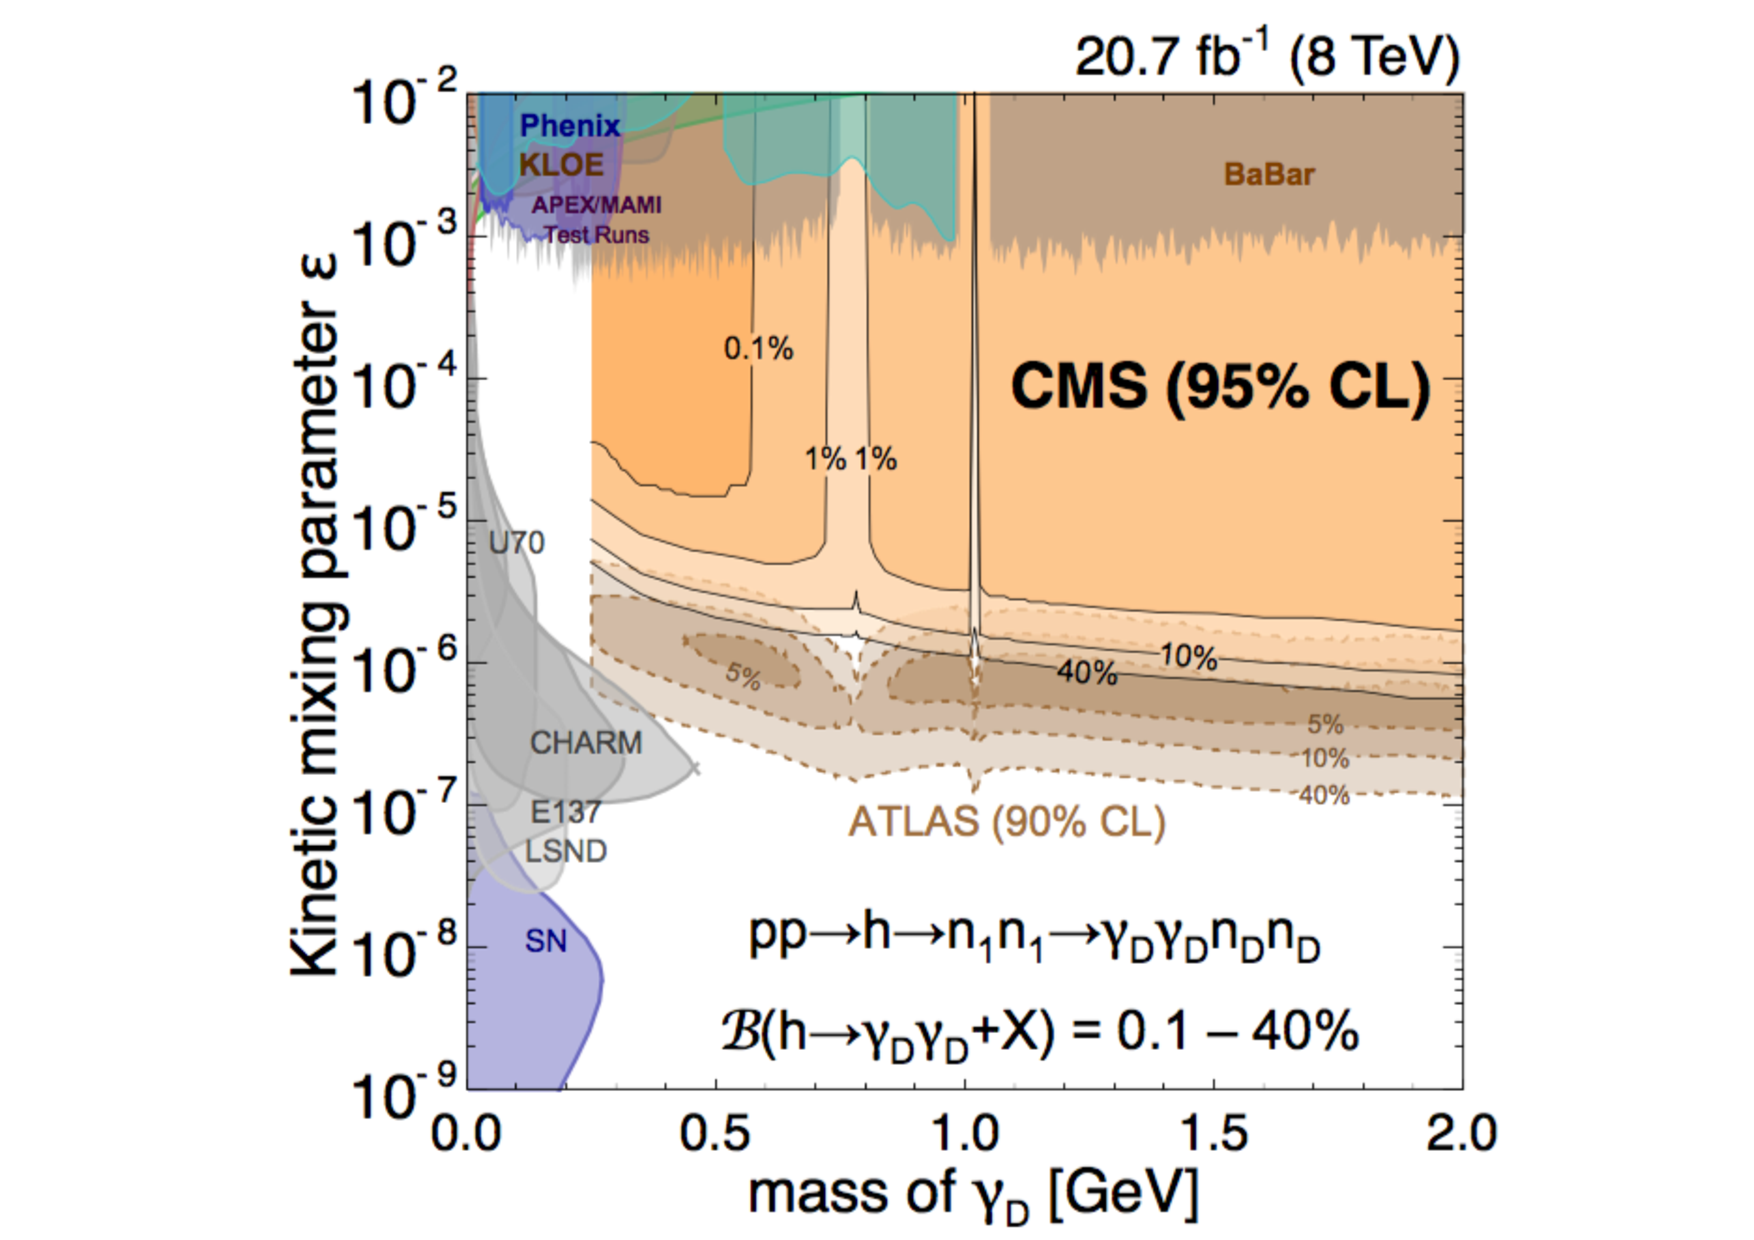
\includegraphics[width=0.9\textwidth]{plots/Limit_Eps_mass_v6.pdf}
\caption{Comparison of the lepton-jet searches at ATLAS~\cite{Aad:2014yea} and CMS~\cite{Khachatryan:2015wka} with respect to a dark photon scenario~\cite{Falkowski:2010cm} vis-a-vis dark photon limits coming from low-energy experiments. Figure taken from Ref.~\cite{Khachatryan:2015wka}.}
\label{fig:dark_photons_CMS_ATLAS}
\end{figure}

\subsection{Summary}
\label{sec:leptonicsummary}

To summarize, the lepton searches rely on fairly standard lepton identification, with vertex reconstruction being performed mostly offline. Searches for leptonically decaying LLPs typically enjoy low trigger thresholds and good sensitivity to LLP production rates. Extending the success of the leptonic LLP program to future LHC running will necessitate maintaining low-threshold triggers for displaced leptons in a high-luminosity environment; this is a major challenge but one that must be overcome. Another outstanding challenge is coverage of LLP decays to $\tau$ leptons, which lie at the interface between hadronic and leptonic searches. Such decays are very well motivated from the theoretical point of view, as a Higgs-like scalar can typically decay about 300 times more often into $\tau^+ \tau^-$ if kinematically allowed, and also one could have large rates into mixed decay modes such as $\tau^+ \mu^-$. A displaced hadronic $\tau$ is a striking object, and most likely will have few backgrounds. Hence, limits on exclusive displaced $\tau$s would be of utmost importance~\footnote{We note that if the $\tau$ originates from outside the tracker, the hadronically decaying taus are indistinguishable from other displaced hadrons. For instance, in the ATLAS search utilizing muon RoIs~\cite{Aad:2015uaa} the results are interpreted for a model with a scalar particle with Higgs-like couplings to SM fermions, which includes a branching fraction into $\tau^+ \tau^-$. However, if the $\tau$ originates from the ID, the low number of tracks associated to it (one to three) will not fulfill the requirements of the ATLAS study of five or more tracks associated to a DV.}.

As the leptonic searches explicitly require opposite-sign leptons, the same-sign lepton signature (motivated from Majorana neutrinos; see the LHCb search in Section~\ref{subsec:dsemilep}, or heavy, doubly-charged LLPs) is currently neglected. Furthermore, the sensitivity of the CMS search for two high-$|d_0|$ leptons is currently only sensitive to opposite sign $e\mu$ pairs, with a veto on additional leptons. Relaxing these requirements would greatly enhance sensitivity to certain scenarios, especially the simplified models with flavor-conserving leptonic LLP decays.

Lepton-jet searches currently cover only final states with at least two LLPs and some muons in the final state~\footnote{The ATLAS 8~TeV search~\cite{Aad:2014yea} included a search channel with two electron-only lepton-jets, but the performance was poor and it was excluded from the final result.}, and the same statement currently applies to both the LHCb searches for dark photons~\cite{Aaij:2016rxn,Aaij:2017rft} and for LLPs produced in $B$-meson decays. The existing ATLAS lepton-jet studies express their results in terms of specific dark photon models~\footnote{Recall that the lepton-jet studies also consider the $\gamma_D \to \pi^+ \pi^-$ decay mode.}, which makes it complicated to apply the results to other models. We refer the reader to Sec.~\ref{sec:reint} for a further discussion of this topic. In extending lepton-jet searches, it would be beneficial to have additional searches with a single lepton-jet or low-mass, leptonically-decaying LLP (which are motivated in models with hidden sectors and Majorana neutrinos, for example in Refs.~\cite{Izaguirre:2015pga,Izaguirre:2015zva}). In addition, the status of coverage in the intermediate mass-transition region between ``standard" displaced lepton pairs and lepton-jets is unclear, and may potentially harbor a gap; adopting the simplified model approach for leptonic LLP decays with masses varying between the GeV and weak scale would ensure comprehensive coverage of low-mass leptonically decaying LLPs.

Finally, we comment on gaps in sensitivity to very low-mass leptonically decaying LLPs. A benchmark LLP model is the heavy neutral lepton (HNL), which corresponds to the charged-current production mode with (semi-)leptonic LLP decays in our simplified model framework. HNLs constitute an important physics case that leads to multi-lepton displaced signatures from $W$ decays, with nice prospects at ATLAS and CMS~(see, e.g., Refs.~\cite{Izaguirre2015,Nemevsek:2018bbt,Cottin:2018kmq}). While previous searches were not sensitive to this scenario due to either high-\pT requirements or the requirement of two DVs in the same event, the presence of a prompt lepton from the $W$ allows the relaxation of these requirements in a dedicated analysis.  Moreover, the prospects of triggering on a prompt lepton in such searches was studied recently in Ref.~\cite{Cottin:2018kmq} and demonstrated in a prompt search in Ref.~\cite{Sirunyan:2018mtv}~\footnote{Note that the displaced large transverse impact parameter $e\mu$ CMS search~\cite{CMS-PAS-EXO-16-022} fails to cover this scenario due to the aforementioned lepton veto, which kills the tri-lepton signals discussed in Ref.~\cite{Izaguirre2015}, as well as relatively high lepton $p_T$ trigger thresholds compared to the kinematics of 4-body $W$ decay.}. The identification of two leptons from the vertex is a powerful discriminant against backgrounds from meta-stable particle decays and hadronic interactions in material. This permits a potentially cleaner exploration of the lower HNL mass range (3--6~GeV) than in the semi-leptonic channel (see Section~\ref{subsec:dsemilep}) despite the lower branching ratio. It should be noted that HNL models can predict LLP decays to all three lepton flavors (either democratically or hierarchically), necessitating the capability to reconstruct displaced leptons of all flavors, including taus.

\section{Semi-Leptonic Decays}
\label{subsec:dsemilep}

As semi-leptonic signatures include aspects of both hadronic and leptonic LLP decays, many of the previously discussed searches can partially cover these cases, and some do so explicitly. For instance, the ATLAS search for electrons and muons accompanied by tracks~\cite{Aad:2015rba}, the inclusive CMS search for DVs~\cite{Sirunyan:2017jdo} (which contains a specific model interpretation called ``$B$-lepton'' addressing precisely this channel), and the search for a large impact parameter $e\mu$ pair by CMS~\cite{CMS-PAS-EXO-16-022} are all inclusive with respect to other hadrons produced in the LLP decay, provided the leptons are sufficiently isolated~\footnote{Note that the lepton isolation affects most of the semi-leptonic searches.}. In addition, LHCb has dedicated searches for semi-leptonically decaying LLPs~\cite{Aaij:2016xmb} and semi-leptonic decays of long-lived Majorana neutrinos coming from $B^{-}$ mesons~\cite{Aaij:2014aba}. The two CMS searches~\cite{Sirunyan:2017jdo,CMS-PAS-EXO-16-022} need no further explanation for how they cover semi-leptonic LLPs because of their very inclusive nature (see Section~\ref{sec:CMSleptonic}), but we now describe the rest of these searches in some detail.

\subsection{LHCb Searches}

The LHCb search for semi-leptonic LLP decays selects events with a muon trigger, then reconstructs a DV offline~\cite{Aaij:2016xmb}. The results are interpreted in terms of four distinctive topologies: single LLP production in association with a new particle (in this case a gluino), double LLP pair production via direct pair production, Higgs decay, or via squark pair production (heavy parent). The LLP then decays to two quarks and a muon (which maps to the $jj\ell$ simplified model decay). Material regions are vetoed for the DV, which results in the dominant background arising from heavy flavor production either directly or from $W/Z$ decays. The signal discrimination is obtained from a multivariate analysis based on the muon \pT and impact parameter, and subsequently the search is optimized based on the LLP reconstructed mass and the muon isolation. This study is sensitive to low-mass LLPs with lifetimes between 1.5 and 30~mm, as can be seen in Figure~\ref{fig:lhcbsemi-leptonic}.
%
\begin{figure}[htb]
\centering
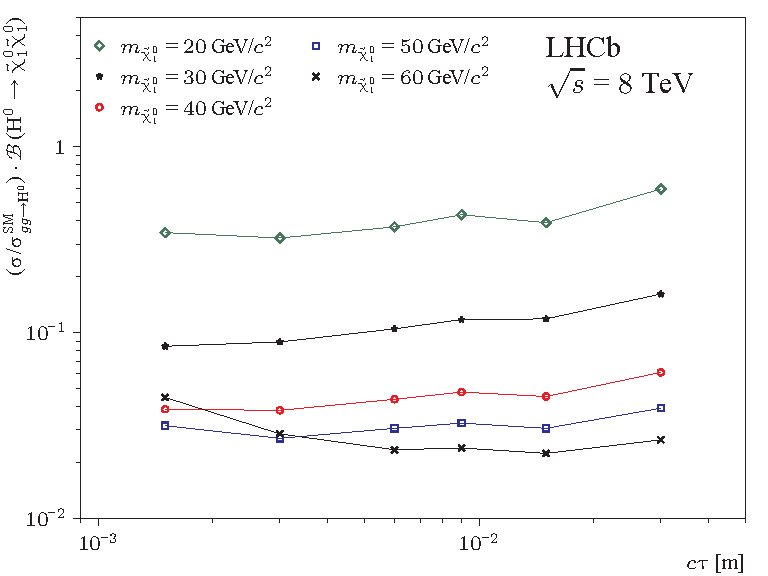
\includegraphics[width=0.9\textwidth]{plots/PAPER-2016-047_sup1.pdf}
\caption{LHCb reach for displaced semi-leptonic decays. Taken from Ref.~\cite{Aaij:2016xmb}.}
\label{fig:lhcbsemi-leptonic}
\end{figure}

The LHCb search for Majorana neutrinos~\cite{Aaij:2014aba}, $N$, probes Majorana neutrinos produced in leptonic $B$ decays, $B^\pm \rightarrow \mu^\pm N$. The Majorana neutrino subsequently decays exclusively to $N \rightarrow \mu^\pm\pi^\mp$; both prompt and displaced decays are considered~\footnote{Some care is required in interpreting the results of the search on a model with a Majorana neutrino, as the original theory interpretation is problematic~\cite{Shuve:2016muy}.}. A same-sign muon requirement, along with the reconstruction of the $N$ and $B$ meson masses, greatly reduces backgrounds to the search. The sensitivity of the search is limited by the restriction to muons in the final state (so models that predominantly decay to $e$ or $\tau$ are not constrained), and the same-sign lepton requirement gives sensitivity only to lepton-number-violating processes. More inclusive searches looking for additional $N$ production modes~\cite{Gorbunov:2007ak}, decays with opposite-sign leptons, or searches targeting decays of heavier mesons like $B_c$~\cite{Milanes:2016rzr} could also improve the sensitivity to semi-leptonically decaying LLPs.

\subsection{ATLAS Search}

The ATLAS search for semi-leptonic LLP decays~\cite{Aad:2015rba} looks for a vertex with a lepton accompanied by tracks. This search uses the same trigger as the dilepton vertex search described in Sec.~\ref{subsec:dleptons}. The DV is required to have a lepton as well as at least four additional associated displaced tracks, and the invariant mass of the tracks must exceed 10~GeV. Thus, the search in principle can have sensitivity down to masses $\gtrsim$~10~GeV, although the high \pT threshold for the displaced electron/muon typically limits sensitivity to low-mass LLPs; the vertex must contain a muon with $\pT >$ 55~GeV or an electron with $\pT >$ 125~GeV.

\subsection{Summary}

When considering the application of inclusive hadronic or leptonic searches to semi-leptonic LLP decays, it is important to understand how the simultaneous presence of leptons and jets in the signal can degrade the sensitivity. For instance, prompt jet searches explicitly can remove non-standard jets through jet cleaning cuts. Lepton isolation criteria can severely reduce the signal acceptance for a highly-boosted LLP decaying into a lepton and a jet, and they might also veto extra tracks in the events. Thus, boosted semi-leptonic decays (as might be found in the displaced decay of a low-mass, right-handed neutrino produced via $W$ decay) may not be covered by existing searches.

One of the major gaps in semi-leptonic LLP searches is at the smallest LLP masses. In this case, it can be challenging for the leptons from LLP decays to pass trigger thresholds and/or isolation criteria; backgrounds from heavy-flavor and other processes are also higher for semi-leptonic processes than fully leptonic ones. However, there are very good motivations for low-mass semi-leptonic LLPs from the HNL benchmark model~\footnote{In the language of simplified models, this corresponds to the charged-current production mode, where the HNL LLP is produced in association with a prompt lepton. The HNL then decays semi-leptonically via the $jj\ell$ channel.} introduced in Sec.~\ref{sec:leptonicsummary}, which predicts LLPs for HNLs of masses below 30~GeV. The signature of HNLs from $W$ decays with displaced semi-leptonic HNL decays is an important item on the search agenda of ATLAS, CMS and LHCb~\cite{Helo2014,Izaguirre2015,Mermod2017,Antusch2017,Nemevsek:2018bbt,Cottin:2018kmq}. The semi-leptonic channel has the highest branching ratio (about 50\% in the relevant mass range~\cite{Gronau1984}) and can therefore offer the best discovery prospects at LHC experiments for HNL masses up to 30~GeV as long as a DV mass cut of around 6~GeV is made to mitigate backgrounds from B-mesons, $m_B \sim$ 5~GeV, and backgrounds from random-crossings can be suppressed. The lower end of the 6--30~GeV mass range corresponds to a non-perturbative regime for the hadronization of the HNL decay products. As the number of charged hadrons significantly affects the DV reconstruction efficiency, the validation of event generator outputs for this process is an important issue currently being addressed by the community (see e.g., Ref.~\cite{Cottin:2018kmq}). The ability of LHCb to trigger directly on the HNL decay products and better reconstruct displaced tracks can in some cases compensate for its lower acceptance and luminosity, as exemplified by a recent search for DVs composed of one muon and several tracks~\cite{LHCb2017,Antusch2017}. This possibly enables LHCb to better probe the more challenging tau channel. Figure~\ref{fig:HNLsensitivity} shows the overall expected reach of LHC searches in the HNL coupling strength (for the muon channel) versus mass plane, using assumptions detailed in Ref.~\cite{Mermod2017}, similar to those in Refs.~\cite{Helo2014,Izaguirre2015}.

\begin{figure}[th]
\centering
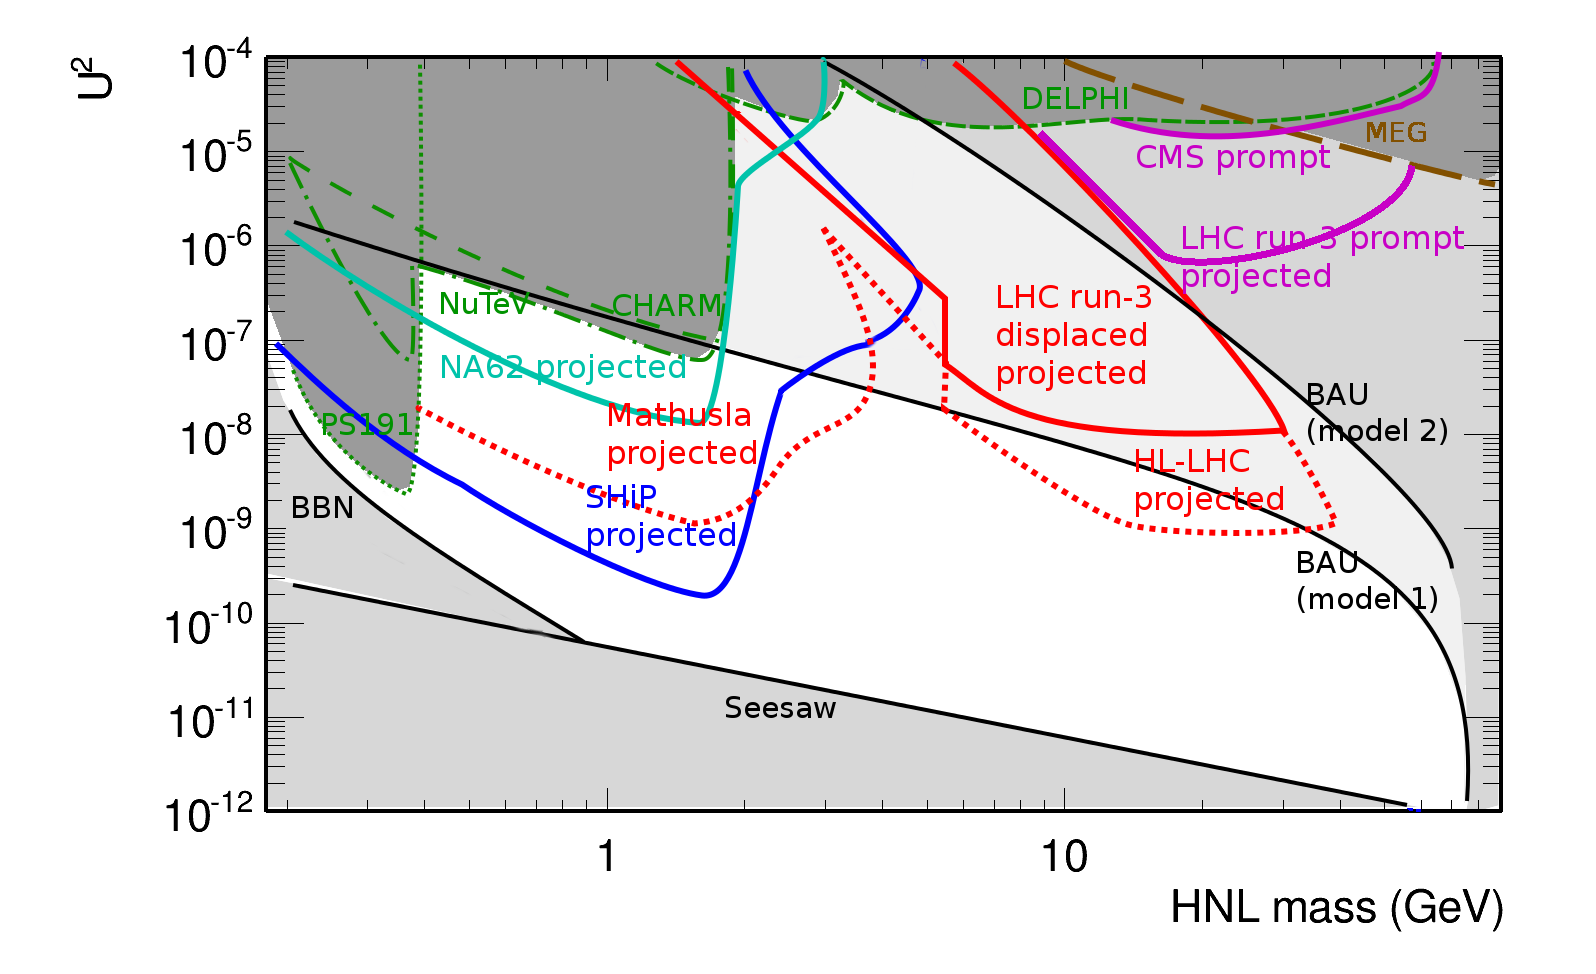
\includegraphics[width=0.99\linewidth]{plots/BigPicture.png}
\caption{Summary of projected experimental sensitivities to HNLs in various experiments, in the coupling strength ($U^2$ for dominant mixing to $\nu_\mu$) vs. mass plane. The projections labelled ``LHC run-3'' and ``HL-LHC'' are for HNLs in $W$ decays in general-purpose experiments, and the one labelled ``Mathusla'' assumes the full HL-LHC MATHUSLA dataset. We also show the recent CMS result for the prompt tri-lepton signature~\cite{Sirunyan:2018mtv}. Prospects at proton beam-dump experiments are also shown for an already existing experiment, NA62~\cite{Lanfranchi2017}, and for the planned experiment SHiP~\cite{SHiP2015}. Direct~\cite{Bernardi1988,CHARM1986,NuTeV1999,Delphi1997,CMS2015b} and indirect~\cite{MEG2013,Antusch2015} limits are indicated as dashed green and brown lines respectively. The lines labelled ``Seesaw'' and ``BBN'' show lower theoretical constraints from the observed neutrino masses (assuming a normal hierarchy) and primordial nucleosynthesis, respectively~\cite{Canetti2013b}. The lines labelled ``BAU'' are upper theoretical constraints from two different models accounting for baryon asymmetry in the universe: model 1 requires the lightest HNL to be a dark matter~\cite{Canetti2013b} candidate, while model 2 allows for all three HNLs to participate in leptogenesis~\cite{Canetti2014}. In particular models, it may be possible to obtain an asymmetry in the entire parameter space up to the CMS Prompt limit {\bf (cite Marco?)}. }
\label{fig:HNLsensitivity}
\end{figure}

The sensitivity of LHC experiments to HNLs is complementary to that of fixed-target experiments which can probe lower couplings thanks to high-intensity beams albeit at lower mass ranges (i.e., targeting HNLs from $c$ and $b$ decays). The CERN SPS provides great opportunities with the running NA62 experiment~\cite{NA622017a} and the planned SHiP experiment~\cite{SHiP2015}, which comprise a vacuum decay vessel and spectrometer tracker downstream of the target to reconstruct vertices of long-lived neutral particles~\footnote{The proposed detector FASER would also have the capability to reconstruct such vertices~\cite{Kling:2018wct}.}. These provide the best sensitivity to HNL masses up to 2~GeV, where they probe a region of the parameter space favored in models which simultaneously explain neutrino masses, matter-antimatter asymmetry and dark matter~\cite{Asaka2005b,Canetti2013b,Mermod2017b,Drewes:2017zyw} (see Figure~\ref{fig:HNLsensitivity}).

\section{Photonic decays}
\label{subsec:dphotons}

There are two ways in which photons coming from LLP decays do not resemble standard photons. First, they cannot be traced back to the PV, thus giving rise to \emph{non-pointing} photons. Second, they can arrive at the ECAL at a time slightly later than expected because the LLP moves slower than the speed of light; these are referred to as \emph{delayed} photons. We note that both kinds of unusual photons can be vetoed in searches for photons that originate from the PV, and thus prompt searches typically provide weaker bounds on LLP scenarios than for promptly decaying signals. ATLAS has a search for non-pointing and delayed photons~\cite{Aad:2014gfa} using the full 8~TeV dataset, which supersedes the 7~TeV analysis~\cite{Aad:2013oua}. In CMS there are studies for delayed photons in the ECAL~\cite{CMS:2015sjc} and for non-pointing photons detected via their conversion to $e^+ e^-$ pairs~\cite{CMS:2015gga}. The underlying topology in all these models is the neutralino decay into a gravitino and a photon ($\chi^0_1 \to \gamma \tilde{G}$), ubiquitous in gauge-mediated supersymmetry breaking (GMSB) scenarios~\cite{Dine:1994vc,Giudice:1998bp}. Hence all these studies require large $\metm$ in the final state. This corresponds to heavy parent production of LLPs with decays to a single photon and \met in the simplified model framework; all searches described below use the Snowmass Slopes Point 8 benchmark, which is not straightforward to map to a physical spectrum of heavy parent masses.

\subsection{ATLAS Search}

The ATLAS study~\cite{Aad:2014gfa} benefits from the capability of the liquid-argon electromagnetic calorimeters to measure the flight direction and the time-of-flight of photons. Resolutions on $\Delta z_\gamma$, the separation between the PV of the event and the extrapolated origin of the photon, and $|\Delta t_\gamma|$, difference of the arrival time of the photon with respect to the prompt case, are as low as 15~mm and 0.25~ns, respectively. The trigger demands two photons within $|\eta| <$ 2.5, with transverse energies $E_T$ of 35 and 25~GeV. In addition, to guarantee the event comes from a proton--proton collision, a PV with five or more tracks with $\pT >$ 0.4~GeV is required. The offline selection requires two photons with $E_T >$ 50~GeV and $|\eta| <$ 2.3, not in the barrel-endcap transition region (1.37 $< |\eta| <$ 1.52), at least one of them in the barrel ($|\eta| <$ 1.37) and with less than 4~GeV of energy deposited in the calorimeter in a cone of $\Delta R$ = 0.4 around them (consituting the \emph{isolation} criterion). In addition, the events are binned in $\metm$: the $\metm <$ 20~GeV bin contains the prompt backgrounds, the 25~GeV $< \metm <$ 75~GeV bin is used as the control region, and finally the signal analysis is performed in the $\metm >$ 75~GeV bin. This study covers lifetimes from 0.25 to 100~ns in the GMSB framework, the lower limit being a hard cut-off imposed experimentally, as the similarity between background and signal samples in that region makes discrimination rather difficult. The excluded signal rates in this range of lifetimes vary between 0.8 and 150~fb, with the best-constrained value obtained for $\tau \sim$ 2~ns.

\subsection{CMS Searches}

The CMS study of delayed photons~\cite{CMS:2015sjc} follows a similar approach to ATLAS. The main difference is that it demands only one photon with $\pT >$ 80~GeV, but in addition two jets are required. Furthermore, the vector sum of \met and $E_T^\gamma$, which is denoted $E_{T~{\rm no}\gamma}^{\rm miss}$, is additionally used for background discrimination. Collisional backgrounds have small \met  and large $E_{T~{\rm no}\gamma}^{\rm miss}$, while the non-collisional backgrounds are characterised by large \met and small  $E_{T~{\rm no}\gamma}^{\rm miss}$. For the signal events the two variables are large, hence they are both requested to be larger than 60~GeV. The time resolution is 0.372~ns, slightly worse than in the optimal scenario of the ATLAS search. Their reach in lifetimes lies in the 2--30~ns range, excluding signal rates of 10--30~fb.

The CMS study of non-pointing photons~\cite{CMS:2015gga} relies on the photon converting to $e^+ e^-$ pairs. It requires two photons, two additional jets, and $\metm >$ 60~GeV. The photon trajectory is obtained from the conversion vertex as the line segment along the momenta of the $e^+ e^-$ track pair, and the impact parameter, $|d_{XY}|$, is defined as the closest distance between the photon and the beam axis, which can be determined within approximately 1~mm. A comparison of the reach of these 8~TeV studies, as well as those using the 7~TeV dataset, can be found in Figure~\ref{fig:gaga}.

%%%%%%%%%%%%%%%%%%%%%%%%%%%%%%%%%%%%%%%%%%%%%%%%
\begin{figure}[htb]
\centering
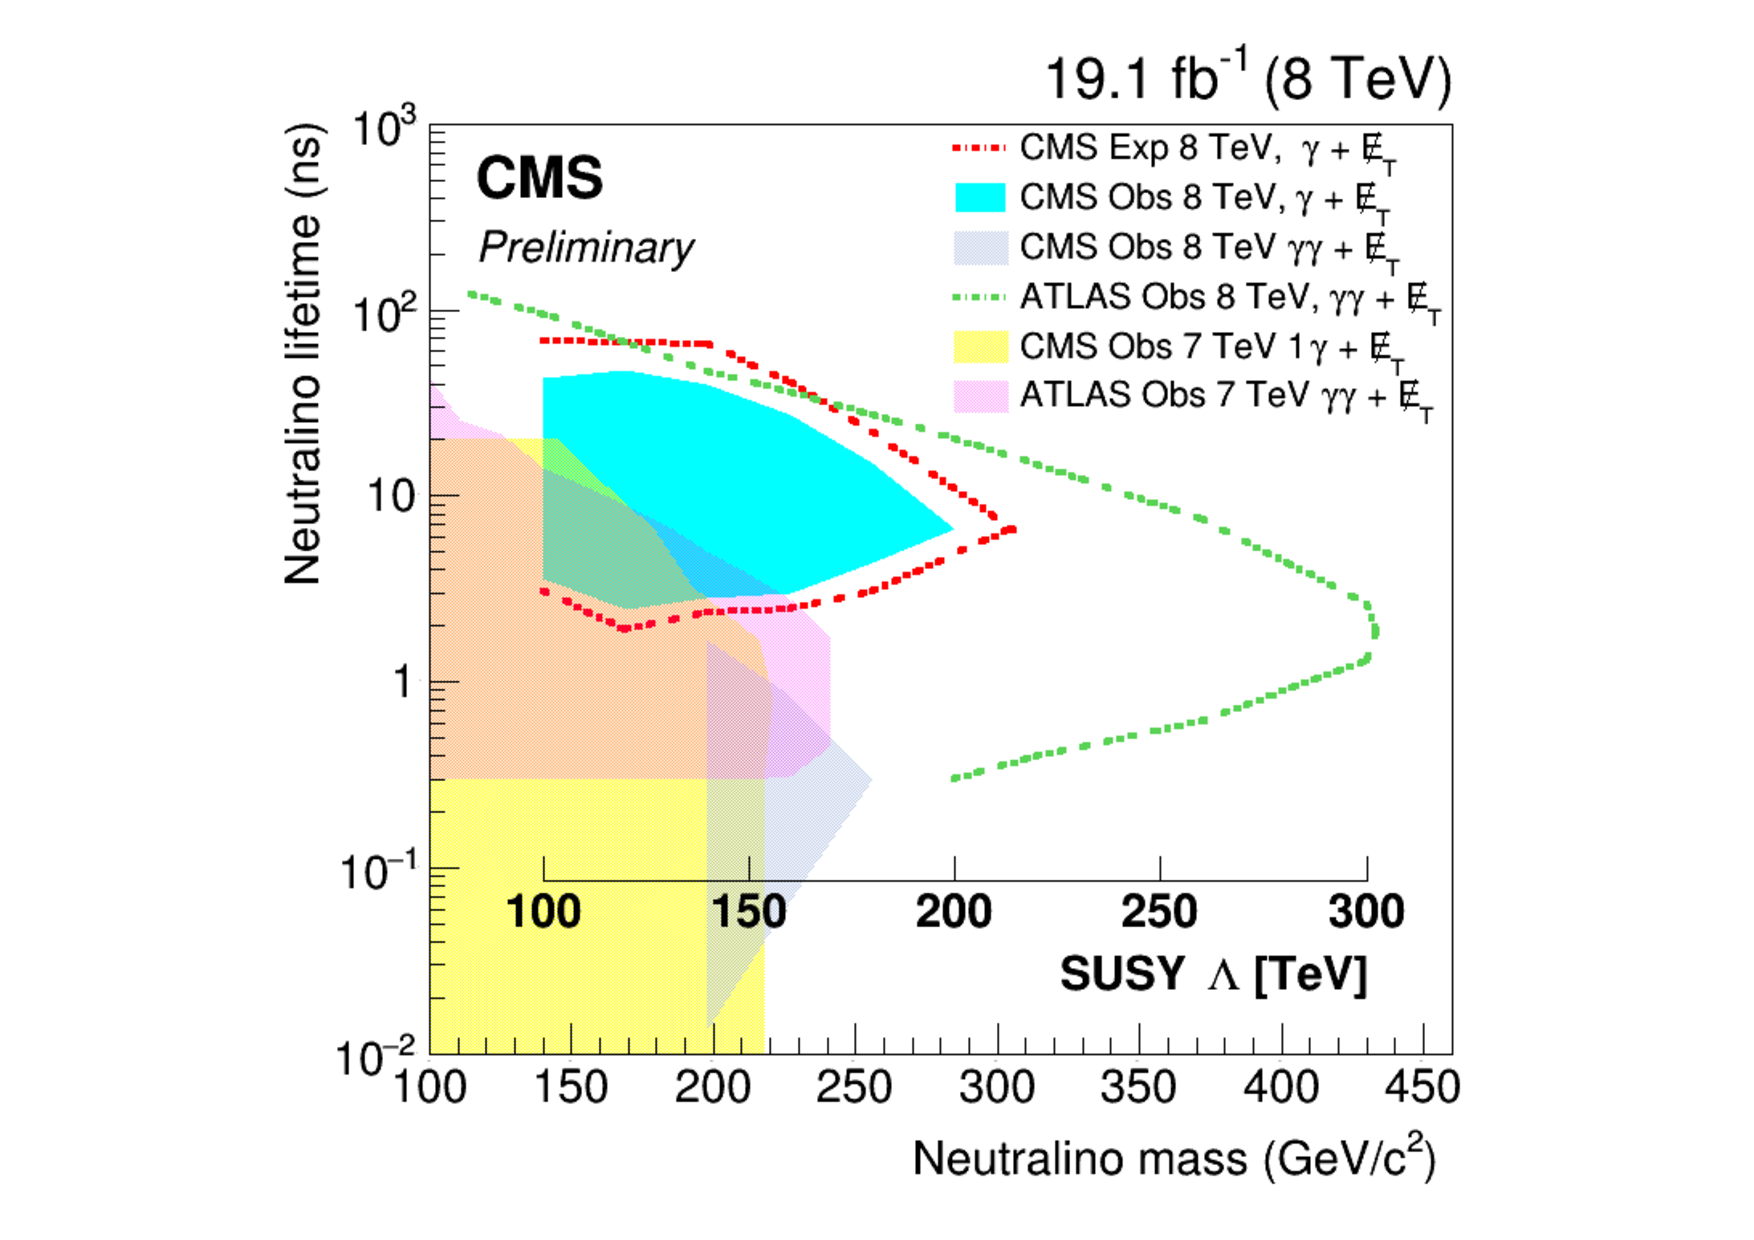
\includegraphics[width=0.9\textwidth]{plots/CMS-PAS-EXO-12-035_Figure_016-a.pdf}
\caption{Summary of the $\gamma + \metm$ searches from ATLAS and CMS, displayed assuming the same GMSB model. Taken from Ref.~\cite{CMS:2015sjc}. }
  \label{fig:gaga}
\end{figure}
%%%%%%%%%%%%%%%%%%%%%%%%%%%%%%%%%%%%%%%%%%%%%%%

\subsection{Summary}

The gaps in these studies are straightforward to identify. The requirement of large $\metm$ is due to the fact that all of these studies have an underlying theoretical picture of neutralinos decaying into gravitinos and photons, motivated from GMSB scenarios. Hence, these searches do not cover cases without the presence of missing energy, including LLPs that decay to $\gamma \gamma$, $l \gamma$ or $j \gamma$. It may be possible to extract a constraint on such LLP decay modes due to mis-measurement of jets or the photon decay geometry which could mimic large missing energy; however, this would be sub-optimal compared to a dedicated search. With the exception of the CMS study~\cite{CMS:2015sjc} which requires two additional hard jets, all of these analyses require two displaced photons. A single displaced photon signature can occur in motivated models:~it can easily arise, for example, from a very slightly mixed electroweak triplet and singlet as in SUSY theories (see the UV models in Sec.~\ref{sec:simplifiedmodel}). Furthermore, as discussed in Sec.~\ref{subsec:djets}, a single LLP in the detector can also arise for very large lifetimes of neutral LLPs, which limits the reach of current searches at longer lifetimes. In such scenarios, it is possible that the photons from LLP decay can be quite soft, and obtaining sensitivity to models with single photons from LLP decay and/or low momenta may require triggering on associated prompt objects, similar to the recommendations in Sec.~\ref{sec:hadronicsummary}.

\section{Other exotic long-lived signatures}
\label{subsec:funnytracks}

In the preceding sections, we presented analyses sensitive to LLPs decaying into objects such as jets, leptons, and photons. In many cases, however, LLPs give rise to signatures that are completely distinct from more conventional prompt signatures. In this section, we present analyses that exploit properties of other exotic long-lived signatures, such as non-standard tracks. We summarize in detail the existing searches for heavy, stable charged particles (HSCP); disappearing tracks (DT); stopped particles (SP) and monopoles, and describe existing ideas on how to look for quirks and SIMPs (Strongly Interacting Massive Particles).

Note that the terminology employed in some of these searches can be confusing, with occasional conflation of signatures with the underlying model. We provide a detailed explanation of each search, and we attempt a classification here based strictly on signature. We distinguish between three classes of signals: \emph{tracks with anomalous ionization}, \emph{tracks with anomalous geometry}, and finally \emph{out-of-time} decays.

\subsection{Tracks with Anomalous Ionization}
\label{sec:anomalousionize}

In this category, we collect all searches for charged-particle tracks with anomalous ionization, i.e., those that are inconsistent with a charge $|Q|=e$. Here we include i) the so-called heavy, stable charged particles (HSCPs), which apply to stable, electrically charged particles but also charged particles that decay in the calorimeters and/or MS; and ii) magnetic monopoles.

\subsubsection*{Heavy Stable Charged Particles (HSCPs)}
\label{subsec:ExpHSCP}

The searches for HSCPs at CMS~\cite{Chatrchyan:2013oca,CMS:2016ybj} and ATLAS~\cite{ATLAS:2014fka,Aaboud:2016uth} rely on two key properties. First, particles that are massive and/or electrically charged with $|Q| \ne e$ have a characteristic ionization loss ($dE/dx$) distinctively different than SM particles. This property can be measured in the tracker. Second, HSCPs are typically heavy and move with a speed less than the speed of light, $\beta = v/c <$ 1. Thus, compared to a particle with $\beta \approx$ 1, they require a longer time-of-flight (TOF) to reach the outermost components of the detector (calorimeters and muon chambers). As decays or interactions of the HSCP with the material in the detector can change the electric charge of the HSCP, both CMS and ATLAS perform separate \emph{tracker-only} and \emph{tracker + TOF} studies in the language of CMS~\footnote{ATLAS measures $\beta \gamma$ from $dE/dX$ and $\beta$ from time-of-flight and extracts an independent mass, $m_{\beta}$ and $m_{\beta \gamma}$, from each measurement.}. The event selection relies on standard single-muon or large-missing-energy triggers. The offline selection relies on identifying the signal events from quality requirements on the tracks using discriminator variables built from track observables.

The HSCP search conducted by LHCb~\cite{Aaij:2015ica} is slightly different. Instead of exploiting $dE/dx$ and time-of-flight, they use the lack of radiation in the ring imaging Cherenkov detector (RICH). Events are required to pass a high-\pT single muon trigger ($\pT(\mu) >$ 15~GeV). Two opposite sign ``muons'' are then required, each with \pT above 50~GeV and an invariant di-muon mass above 100~GeV, to suppress muons coming from DY production, the main background for this search. In addition, particles must have $\beta >$ 0.8, set by the efficiency of the muon chambers to reconstruct slow particles. As electrons and hadrons interact more with the calorimeter than an HSCP, a deposit in the calorimeter of less than 1\% of the momentum of the particle is required.

The theoretical interpretation of a signal or limit depends on whether the HSCP carries both color and electroweak charges. If it carries a color charge, the default benchmarks correspond to $R$-hadrons, namely HSCPs that hadronize with SM particles via the strong force, e.g., gluino-gluon or quark-squark states. In the absence of a color charge, the signal is exemplified by long-lived sleptons in the context of gauge-mediated SUSY. Both ATLAS~\cite{ATLAS:2014fka} and CMS~\cite{CMS:2016ybj} studies employ these two scenarios, while LHCb~\cite{Aaij:2015ica} uses a stau benchmark model~\footnote{The ATLAS R-hadron searches using the 13~TeV dataset have recently been presented in Ref.~\cite{Aaboud:2016uth}. }.
Finally, CMS also looks for HSCPs coupling only to hypercharge (and hence possessing only couplings to $\gamma$ and $Z$), while ATLAS has a search inspired by electroweakinos in SUSY:~it considers the associated production of a neutral and an electrically charged LLP (chargino-neutralino), and thus only one HSCP plus missing energy are required. These scenarios correspond, in our simplified model framework, to the direct production of LLPs with electric or color charges and that do not decay, or decay at very large distances compared to the tracking volume.

To summarize, these searches present no obvious weak points. Standard triggers and tracking algorithms are used, and the analysis methods are well-understood and have been extensively validated against data. HSCP signatures do not suffer from the low-mass gap of many neutral LLPs due to constraints from LEP and other low-energy experiments. However, milli-charged particles are not covered by these searches and require dedicated detectors (see Sec.~\ref{sec:milliQan}). While the HSCP search strategies are generally robust, we encourage the experimental collaborations to continue pursuing improvements for these searches. The small number of signal events that would be produced for HSCPs above current limits render the sensitivity highly dependent on the understanding of the background and control of the systematics.

\subsubsection*{Magnetic Monopoles}

ATLAS~\cite{Aad:2015kta} has a dedicated search for highly ionizing particles (HIPs), which encompass a variety of new physics scenarios, such as magnetic monopoles, dyons (particles with both magnetic and electric charge), stable microscopic black holes, etc. For the sake of concreteness, we focus on magnetic monopoles but the interpretation in terms of other models is straightforward.

The main phenomenological feature is that magnetic charge is quantized in units of $g_D = 2\pi/e \approx$ 68.5. Hence, a magnetic monopole behaves as a particle with at least 68.5 electron charges, leading to an unusually large ionization power in matter, so that they would quickly stop in the detector because HIPs lose energy at spectacular rates. Because of the large QED coupling of magnetic monopoles, a perturbative calculation of the cross section is invalid and there is no accurate determination of the production rate, but a na\"ive Drell-Yan production cross section is provided for the purposes of comparison. The specifics of the detector restrict the sensitivity of this search to magnetic charges $g < 2 g_D$ because a large fraction of the monopoles stop in the material upstream of the electromagnetic calorimeter, as the latter is used for the L1 trigger~\cite{DeRoeck:2011aa}. We note that larger magnetic charges can be tested by the MoEDAL experiment~\cite{MoEDAL:2016jlb}, which is described in detail in Sec.~\ref{sec:MoEDAL}.

ATLAS~\cite{Aad:2015kta} has a dedicated trigger for HIPs based on identifying relevant RoIs in the ECAL and subsequently counting the number of hits in the transition radiation tracker (TRT). As well, the fraction of TRT hits that are high-threshold (HT), meaning that they have an ionization larger than $\sim3$ times that expected from a SM particle, is used as a discriminant. The analysis selects events based on the fraction of TRT-HT hits matched to an EM cluster deposit, and how the energy deposits are distributed in the different layers of the ECAL. It is important to note that due to the lack of a consistent theory, the signal simulation is performed by re-scaling Drell-Yan production at leading order and assuming no coupling to the $Z$ boson. The HIPs are assumed to have either spin-0 or 1/2. The spin does not affect the interaction with the material, but the angular distributions are different according to angular momentum conservation (keeping in mind that there is, of course, no perturbative theoretical prediction for the angular distribution). Cross-section limits for 0.5 $< |g|/g_D <$ 2 are set for masses in the 890--1050 (1180--1340)~GeV range for the spin-0 (1/2) case.

The coverage in LHC Run-2 of magnetic monopoles in the $g_D-\sigma$ plane is displayed in Figure~\ref{fig:magnetic_monopole_reach}.
%
\begin{figure}[htb]
\centering
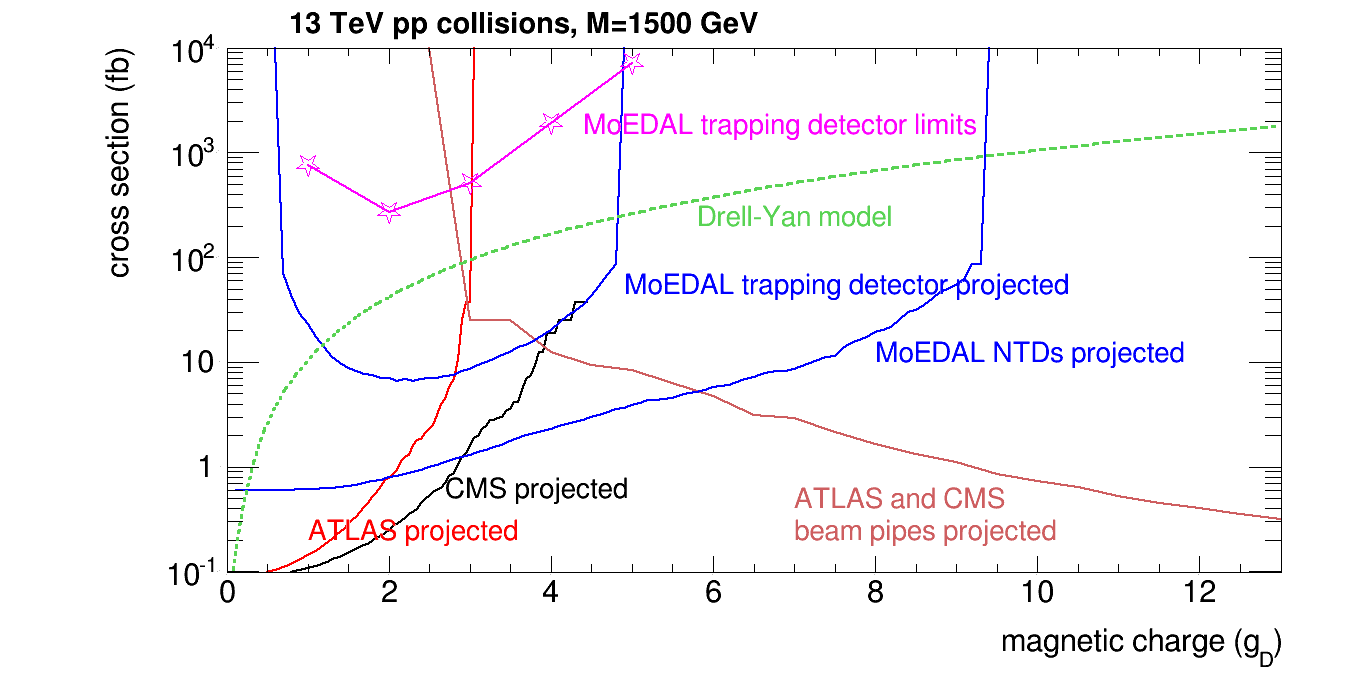
\includegraphics[width=0.9\textwidth]{plots/monopoles_xsec_13TeV_3events}
\caption{Comparison of the MoEDAL, ATLAS and CMS reaches for magnetic monopoles. The curves assume three signal events and a total integrated luminosity of 50~fb$^{-1}$ for 13~TeV collisions. Source: private communication from P. Mermod; updated version of existing figure in Ref.~\cite{DeRoeck:2011aa}.}
\label{fig:magnetic_monopole_reach}
\end{figure}

\subsection{Tracks with Anomalous Geometry}

In this category we group searches where the tracks have an anomalous geometry, namely they disappear (track $\to$ nothing), or follow non-standard trajectories (such as quirks). There are additional anomalous track signatures that we do not cover such as kinked tracks, where a charged LLP decays to another charged particle that travels at a non-zero angle with respect to the LLP direction~\cite{Dimopoulos:1996vz,Hamaguchi:2004df,Asai:2011wy,Jung:2015boa}; however, there are currently no dedicated searches for such signatures. 

Within this category we also have the emerging jets signature that has been recently studied by CMS~\cite{CMS-PAS-EXO-18-001}. Since emerging jets arise dark sector radiation, they are described in detail in Chapter~\ref{sec:showers} in conjunction with the theoretical and phenomenological aspects of dark showers.

\subsubsection*{Disappearing tracks (DT)}

Massive charged particles traveling in the detector can decay to a lighter, almost mass-degenerate neutral state, emitting a soft SM charged particle (typically a pion or a muon). While at first glance a small mass gap na\"ively seems like a hallmark of tuning, near degeneracies often occur naturally as a result of a symmetry. In fact, electroweak symmetry generically leads to small mass splittings between components of a single electroweak multiplet. For example, ${\cal O}$~(100~MeV) splittings arise between the different components of an electroweak multiplet~\cite{Thomas:1998wy,Cirelli:2005uq} due to EW gauge boson loops~\footnote{For a single fermion multiplet, the splitting can only be altered by higher-dimensional operators, and thus it is harder to vary $\Delta$ from the 1-loop EW value. For other cases, such as mixing with additional particles, the actual splitting can differ more substantially from this 1-loop EW value.}. If the SM particle is sufficiently soft it cannot be reconstructed, and then a charged track seems to vanish: this is thus referred to as a disappearing track~\footnote{If the charged particle could be reconstructed this case is often referred to as a \emph{kinked track}. However, as the kinked portion has a very large impact parameter, without a serious attempt to capture the kink these tracks, too, simply disappear.}. The actual lifetime of the charged particle is highly sensitive to the precise value of the mass splitting. For instance, the well studied cases of a fermionic doublet with $Y=1/2$ and a fermionic triplet with $Y=0$, reminiscent of a Higgsino and Wino in supersymmetry, respectively, have mass splittings of $\Delta$ = 355 and 166~MeV, up to small corrections, but the corresponding $c \tau$ values differ by almost an order of magnitude: 6.6~mm versus 5.5~cm~\footnote{While these values set a concrete physics target, we stress again that the mass splitting can be arbitrary in other corners of the BSM parameter space (even within SUSY). For instance, $\tilde{\tau} \to \tau \tilde{\nu}$ (where the stau and sneutrino masses are free independent parameters) or for scalar particles (e.g., $H^+ \to \mu^+ H^0$), where the mass splitting and the overall mass scale are set by arbitrary quartic couplings.}. This is because the lifetime, $c\tau$, depends on the third power of the mass splitting in these scenarios when the charged LLP decays to a charged pion~\cite{Thomas:1998wy,Cirelli:2005uq}.

Before 2017, both ATLAS~\cite{Aad:2013yna} and CMS~\cite{CMS:2014gxa} required a track to travel about 30~cm in order to be reconstructed, giving good coverage of the Wino scenario. This 30~cm value corresponds to four hits at ATLAS, three in the pixel layers plus one in the silicon tracker, and to seven hits in the pixel and trackers of CMS. The search employs a trigger requiring an ISR jet against which the charged particle recoils, along with the presence of large \met. The disappearing track is reconstructed offline and needs to fulfill quality criteria (isolation, \pT threshold, etc.). A phenomenological study~\cite{Mahbubani:2017gjh} has shown that reducing the distance from 30 to 10~cm would give coverage to the elusive Higgsino scenario, moving the expected reach up to 400~GeV, surpassing the expected mono-jet reach of 250~GeV~\cite{Schwaller:2013baa,Low:2014cba,Barducci:2015ffa}. Later, ATLAS presented a study~\cite{ATLAS-CONF-2017-017} using 13~TeV data and exploiting the presence of a new innermost pixel layer (IBL). This addition allows for all four hits to be in the pixel, with the outermost pixel layer now at 12.25~cm, enhancing sensitivity to lower values of $c \tau$. The summary for disappearing tracks at ATLAS for the Wino case can be seen in the left panel of Figure~\ref{fig:ewkinosearches}, while in the right panel we show the constraints for Higgsinos from Ref.~\cite{Mahbubani:2017gjh}. CMS also has a disappearing tracks search using 2015 and 2016 data at a center-of-mass energy of 13~TeV~\cite{Sirunyan:2018ldc}.

\begin{figure}[t]
\centering
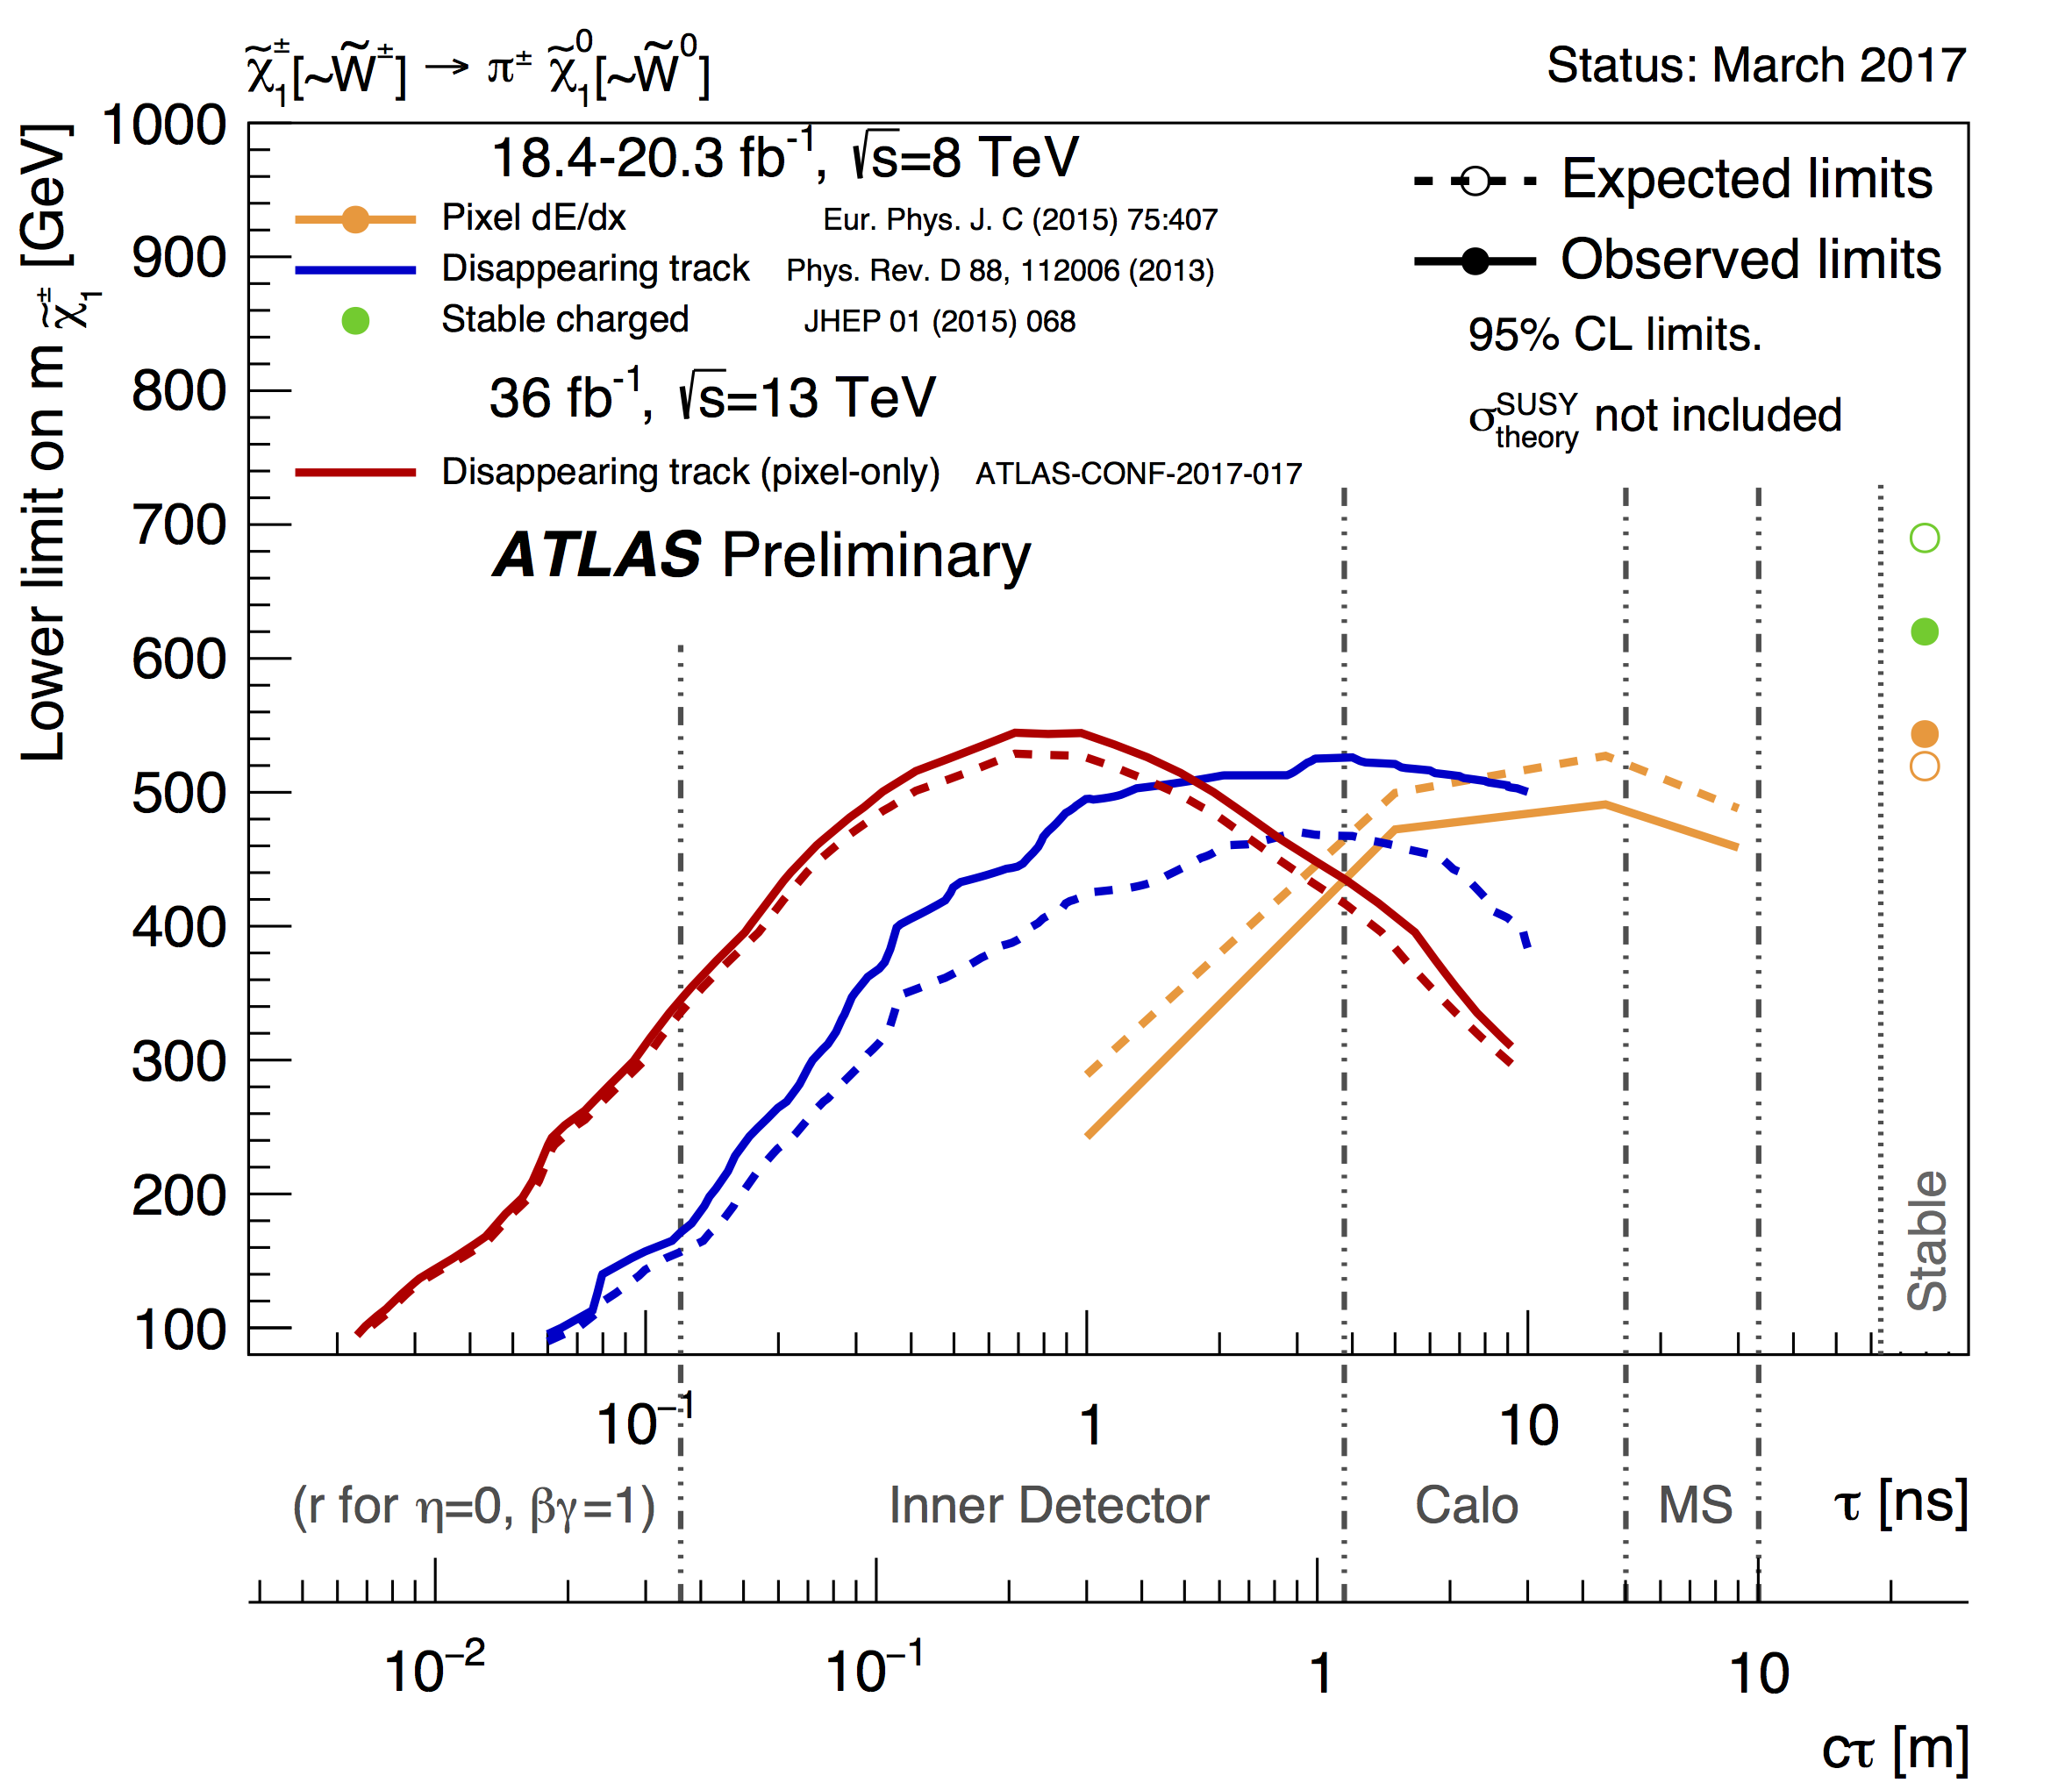
\includegraphics[width=0.44\textwidth]{plots/ATLAS_SUSY_LLPChargino.png}
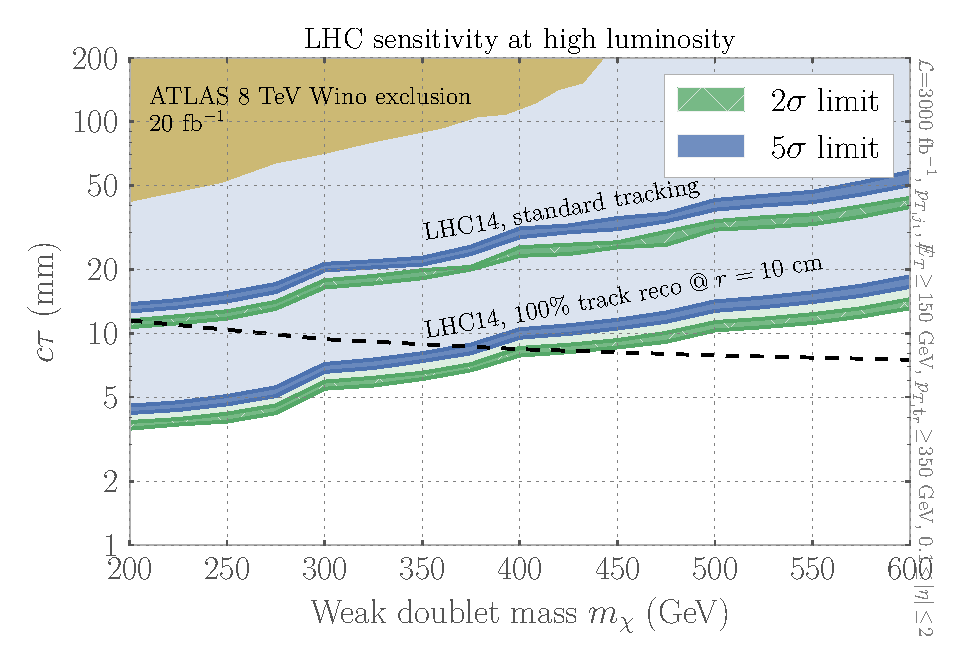
\includegraphics[width=0.54\textwidth]{plots/Higgsino_Significance14}
\caption{Summary of ATLAS disappearing-track searches as applied to a Wino (electroweak triplet) benchmark scenario (left panel)~\cite{ATLAS:summary}; HL-LHC projected constraints on the Higgsino scenario (right)~\cite{Mahbubani:2017gjh}.}
  \label{fig:ewkinosearches}
\end{figure}

At LHCb the prospects for a disappearing track analysis with the present detector are poor. Currently, the momentum of the track can only be measured if the particle passes through the tracking station (TT), which is about 3~m away from the IP. Particles decaying in the VELO or RICH1 system will not leave a fully-measurable track and will be swamped in a background of SM processes such as kaon decays, which would give a similar signature in the detector components before the magnet. Detector improvements (additional magnets, better PID at low momentum, additional layers) might lead to some sensitivity for ${\cal O}$(cm) lived tracks, a golden opportunity for potential LLP discoveries at LHCb in the HL-LHC era.

To summarize, the search for disappearing tracks presents a few challenges. Using an ISR jet trigger means a price is paid in terms of signal efficiency. For example, Ref.~\cite{Mahbubani:2017gjh} has shown that significantly lowering the \pT threshold of the jet or directly triggering on the momentum of the disappearing track~\footnote{While currently there are some proposals to trigger on tracks~\cite{Gershtein:2017workshop}, those only apply to standard tracks. In particular, the new fast track reconstruction (FTK) system at ATLAS requires more than 10 hits~\cite{Holmes:2017workshop,Horyn:2017workshop}.} would lead to a factor of two increase in the number of signal events. It is also clear that better access to lower lifetimes is needed; this may only be possible, for instance, by adding new tracking layers as close as possible to the beampipe (and/or having double layers instead of single ones).

\subsubsection*{Strongly Interacting Massive Particles (SIMPs)}

Strongly interacting massive particles (SIMPs) can be motivated by astrophysical observations of dark matter that do not fully agree with the WIMP paradigm (e.g., missing satellites, the core vs. cusp problem; see, e.g., Refs.~\cite{2010arXiv1009.4505B,2011MNRAS.415L..40B,Weinberg:2013aya,1742-6596-437-1-012001} for further discussion). These particles are assumed to interact strongly with baryons. Consequently, the experimental signature is little to no signal in the tracker and the ECAL, and large energy deposits in the HCAL. Such a final state with trackless jets also arises in the context of emerging jets~\cite{Schwaller:2015gea}, and ATLAS has a trigger for trackless jets in association with a soft muon (where the muon is required to fire L1 of the trigger)~\cite{ATLASLLPTriggers}.% ({\bf \textcolor{red}{JB: Hmm; I think the trackless jet trigger was never used and then removed from the trigger menu, primarily because it wasn't worth keeping because other triggers, like CalRatio, could do its job better for the searches for which it was being used.  Worth checking with Andrea Coccaro, Cristiano Alpigiani and/or Emma Torro, for example.}}).
Additionally, the CalRatio trigger and associated search for displaced hadronic decays (addressed in Section~\ref{subsec:djets}) is designed to be sensitive to a similar signature and could provide some coverage of this signature as well. Strictly speaking, SIMPs are not a track-based signature, but we include them here because the interactions of the SIMPs with the tracker are different from usual hadrons in jets, while the calorimeter signatures are similar.

An LHC phenomenological study of SIMPs was carried out in Ref.~\cite{Daci:2015hca}. We summarize the main points of the study here. In their setup, SIMPs interact with the SM via an attractive potential (either scalar or vector mediator) coupling SIMP pairs to $q\bar{q}$ pairs. The proposed analysis selects events with high-\pT, back-to-back jets within the tracker, exploiting the charged energy fraction within a jet to discriminate signal from background. The astrophysical experimental constraints on this scenario are compared with the expected reach of this search and that of mono-jets in Figure~\ref{fig:simps}. Currently there is an ongoing analysis in CMS pursuing this strategy.

\begin{figure}[t]
\centering
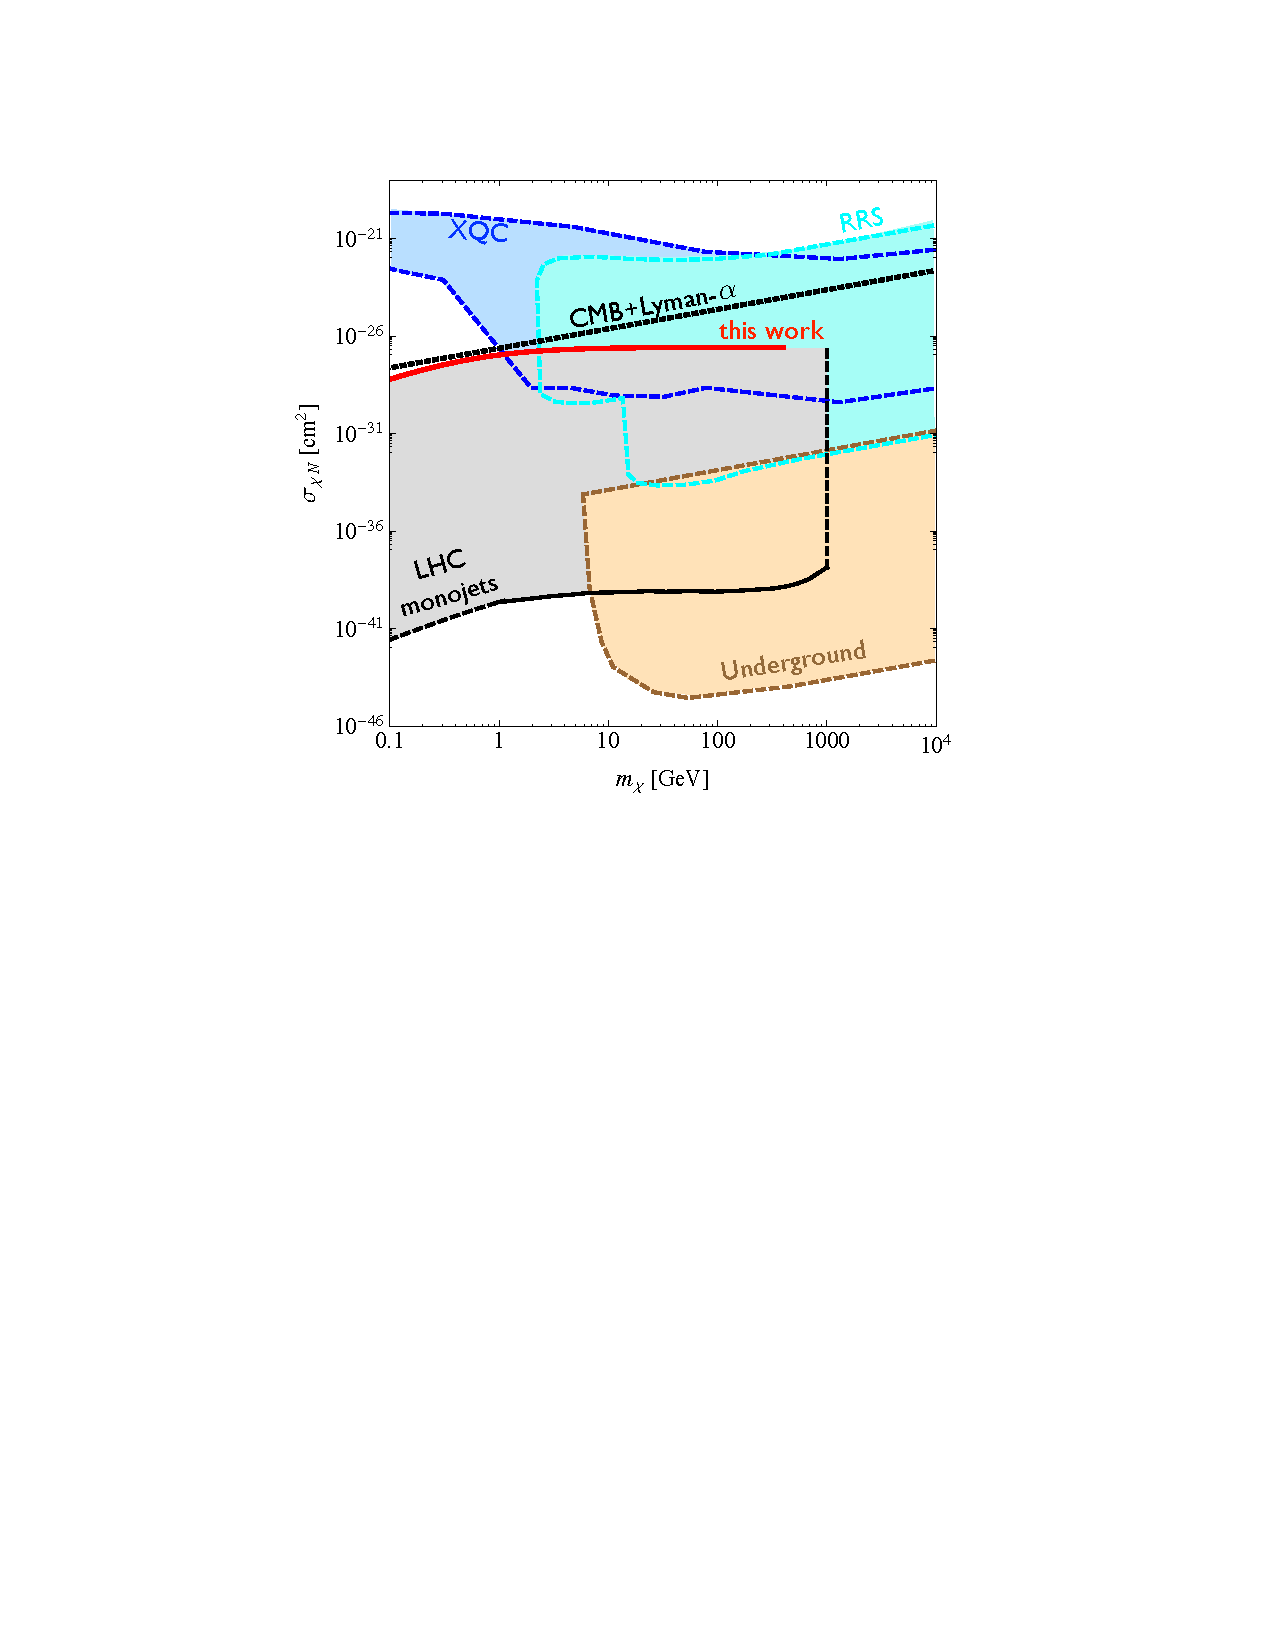
\includegraphics[width=0.9\textwidth]{plots/simps_constraints.pdf}
\caption{Astrophysical and collider constraints on a simple SIMP setup. Note that the relevance of the astrophysical constraints depends on the contribution of the SIMPs to the relic density. Taken from Ref.~\cite{Daci:2015hca}.}
  \label{fig:simps}.
\end{figure}

\subsubsection*{Quirks}

Quirks are particles charged under both the SM and a new confining gauge group~\cite{Kang:2008ea}, referred to here as ``infracolor'' (IC). The defining property of quirks is that the tree-level quirk masses $m_Q$ are above the confinement scale $\Lambda_{IC}$ (and thus similar to QCD but with no light-flavored quarks), so that there is never enough local energy density to pop new quirks out of the vacuum. A pair consisting of a quirk and an anti-quirk can live in a quantum-mechanical bound state where the constituents are separated by macroscopic distances $\ell \sim \frac{m_Q}{\Lambda_{IC}^2}$, remaining connected by an infracolor flux tube. The infracolor flux tube exerts a tension on each quirk that causes its trajectory to differ from the expected helicoidal ones for SM particles. Although well-motivated by hidden-valley models~\cite{Strassler:2006im}, we stress that quirks are not exclusive to hidden valleys, contrary to popular lore.

The collider phenomenology depends greatly on the size of $\ell$.  If $\ell$ is below the mm scale, the individual quirks are not distinguished from one another. However, the pair (which is overall neutral, and therefore does not bend in the magnetic field of the tracker) appears as a single, highly-ionizing straight track with missing energy aligned with it, the latter arising from mis-measuring the track momenta. The $D0$ collaboration has searched for precisely this signature~\cite{Abazov:2010yb}, requesting an additional jet for trigger purposes, finding lower bounds on quirk masses of 107, 119 and 133~GeV for SU(2), SU(3) and SU(5) gauge groups, respectively. However, no extensions of this search to higher mass have been performed at the LHC, and the existing HSCP searches require a fractional uncertainty on the tracks momenta that a straight track cannot provide.

Conversely, if $\ell$ is very large then the existence of the confining force has no effect on the quirk motions, and HSCP searches apply directly to the quirk case, with quirks charged under QCD yielding $R$-hadrons and uncolored quirks leading to slepton-like signatures. We refer the reader to the Sec.~\ref{subsec:ExpHSCP} for more information.

For intermediate values of $\ell$, there are interesting phenomenological prospects at the LHC that have been recently studied theoretically~\cite{Farina:2017cts,Knapen:2017kly}, but for which there are no current public searches by the LHC collaborations. The first study~\cite{Farina:2017cts} has recast mono-jet and HSCP searches, finding bounds up to 1.7~TeV for colored quirk masses. In addition, it has also proposed using the CMS dataset taken with zero magnetic field. In this dataset, all SM particles are expected to follow a straight trajectory, but the quirks would still bend due to the string tension. The second study~\cite{Knapen:2017kly} has proposed a new algorithm to search for quirks, exploiting the fact that the quirk and anti-quirk pair should lie in the same plane with the highest sensitivity in the $\ell \sim$ 1-10~mm range. This avoids the necessity of fitting non-helicoidal trajectories, and has the potential to extend the sensitivity to quirks well beyond the current mono-jet and HSCP limits.

Because of the non-standard nature of the tracks, quirk phenomenology poses substantial challenges in their experimental reconstruction, and the lack of constraints on quirks have already attracted the attention of the ATLAS, CMS and LHCb experiments. It would be desirable to test how the phenomenological proposals in Refs.~\cite{Farina:2017cts,Knapen:2017kly}, among others, can perform in a realistic detector simulation of one of the LHC experiments.

\subsection{Out-of-Time Decays of Stopped Particles}
\label{sec:outoftime}

This category is unique because LLP decays occur out-of-time with the collision. Indeed, decays can even occur when the LHC is not running! The only member of this class is the search for stopped particles, which we describe below.

If an HSCP is produced with very low kinetic energy, it can come to rest in the detector due to interactions with the detector materials. This most likely occurs in the calorimeters or the muon chambers as a result of their high material densities. The HSCP can then decay at a later time when no collision is taking place (referred to as an out-of-time decay). This experimental restriction reduces the types of background processes affecting the search, with the dominant backgrounds coming from cosmic rays, beam halo and instrumental noise.

In the Run-1 analyses from ATLAS~\cite{Aad:2013gva} and CMS~\cite{Khachatryan:2015jha}, events are selected with a dedicated trigger selecting bunch crossings which are empty and have no bunches of protons nearby. The analyses require a jet with \pT ($E$) above 30 (50)~GeV at ATLAS (CMS). ATLAS further supplements the hardware trigger by requiring $\pT(j) >$ 50~GeV, $|\eta| <$ 1.3 and $E_T^{\rm miss} >$ 50~GeV, rejecting instrumental noise. In addition, CMS has updated the jet search in Run-2 and also provided a search that triggers on out-of-time muons, both of which use the 13~TeV dataset~\cite{Sirunyan:2017sbs}. The latter also employs the displaced stand-alone (DSA) muon reconstruction algorithm~\cite{CMS-DP-2015-015}.

An offline selection procedure is aimed at reducing the main backgrounds. Muons coming from cosmic rays can be identified due to their distinctive topology. The ``beam halo'' background is the result of protons interacting with residual gas in the beampipe, the beampipe itself, or collimators upstream from the interaction point. Most particles will not travel far before being absorbed by various structures, but muons will travel parallel to the beam and can leave calorimeter deposits out of time with a proton--proton collision. However, these deposits will often be accompanied by corresponding horizontal tracks in the muon systems and can thus be efficiently vetoed. Instrumental noise is rejected in CMS by exploiting the anomalous response in the HCAL.

Stopped particle searches provide an alternative way of probing charged particles besides more conventional HSCP searches. HSCP searches are typically more sensitive to any signature with a charged particle, so stopped particle searches are not expected to be a discovery mode for most simple new physics scenarios with charged LLPs~\footnote{The reason why the SP searches are less efficient than the HSCP ones is twofold. On one hand, only a fraction of LLPs stop in the detector, while the HSCP search only requires that the LLP crosses the detector. On the other hand, the SP is only looked for in a specific time-window that might fail to catch a large fraction of them.}. The added value of SP searches is that they can help identify and characterise positive signals in HSCPs, for instance by providing a cleaner extraction of the lifetime and also to properly identify the decay products.
%better extraction of the lifetime and the final states).
%({\bf \textcolor{red}{JB: I don't understand this paragraph.  Can someone clarify and re-write?}} {\bf \textcolor{red}{JA:I've tried to clarify a bit. The idea is to explain the complementarity of HSCP and stopped particle searches. Does this help?})
%Moving forward, as luminosity rises and the number of empty bunch crossings per fill decreases it might be worth considering how higher thresholds could control backgrounds and allow for access to novel physics decaying off-time from the rest of the event.

\section{Discovery Opportunities: Overview of Gaps in Coverage}
\label{sec:covgaps}

In the preceding sections (\ref{subsec:djets}--\ref{sec:outoftime}), we have examined the so-called ``coverage'' of existing searches for LLPs at the LHC with the explicit and express purpose of identifying uncovered realms and places where discoveries could be hiding. Here, we summarize these gaps and potential opportunities for LLP discovery in bullet form, as a to-do list for the experimental community.

\begin{enumerate}
\item All-hadronic LLP decays
	\begin{itemize}
	\item Associated-object triggers (especially motivated by Higgs-like VBF and VH production modes) need to be more comprehensively used to improve sensitivity to low-\pT objects
	\item Improvements are needed in sensitivity at lower masses \& lifetimes (e.g., for LLPs produced in Higgs decays)
	\item Single hadronic DVs need to be looked for in searches that currently use two (such as decays in ATLAS HCAL and MS)
	\item Possibilities need to be explored for online reconstruction of hadronic displaced objects, as the inclusive $H_T$ triggers of ATLAS and CMS miss these objects unless they have a large $p_T$. Note that LHCb can actually trigger on a displaced hadronic vertex.
%	({\bf \textcolor{red}{JB: Can we make this explicit with a named example?}})
	\item Low-mass hadronically decaying LLPs can look somewhat like tau leptons, so the question remains as to whether there is any possibility of using, for example, L1 tau triggers to seed displaced jet triggers at HLT and improve trigger efficiency; studies need to be performed by the experimental collaborations
	\item The prospects for dedicated searches for displaced hadronic taus need to be investigated, since no dedicated searches currently exist
	\end{itemize}

\item Leptonic
	\begin{itemize}
	\item Coverage needs to be provided for the intermediate region between boosted, low-mass LLPs (lepton jets) and high-mass, resolved LLPs (resolved ATLAS/CMS searches)
	\item Improvements need to be made to extend coverage to lower masses and to lower \pT thresholds, though currently it's unknown how this can be accomplished, and dedicated studies need to be done
	\item Searches need to be done for different combinations of charge and flavor of displaced leptons (e.g., same-sign vs. opposite-sign, opposite-flavor vs. same-flavor)
	\item Searches need to be done for tau leptons in LLP decays, in particular if they come from the ID; an unanswered question remains as to whether displaced-jet triggers can be used
	\end{itemize}

\item Semi-Leptonic
	\begin{itemize}
	\item Searches do not exist and need to be done for  masses below or about 30 GeV, theoretically well motivated by Majorana neutrinos.
%	({\bf \textcolor{red}{JB: Low-mass whats?  Let's just make it explicit.}}) 
%	($<$~30~GeV, motivated by Majorana neutrinos)
	\item Searches need to be performed for all flavor combinations (for example, one CMS search only covers $e^\pm\mu^\mp$), as well as same-sign vs. opposite-sign leptons
	\item Currently unknown improvements need to be made to relax or modify isolation criteria wherever possible to recover sensitivity to boosted semi-leptonic decays
	\item Searches need to be done that better exploit triggering on associated objects for improved sensitivity to low-mass objects, or to employ high-multiplicity lepton triggers if there are multiple LLPs
	\end{itemize}

\item Photonic
	\begin{itemize}
	\item There is currently no coverage for LLPs decaying into $l \gamma$, $j \gamma$, or without $\metm$, and searches urgently need to be performed for this decay topology
	\item There is currently poor coverage (i.e., there exists no dedicated search) for single-$\gamma$ topologies; the only searches with sensitivity require two jets to be present, and ... needs recasting of CMS delayed photon study~\cite{CMS:2015sjc}.
% ({\bf \textcolor{red}{JB: Actually, I started re-writing this sentence and now I'm not sure what the original sentence is saying.  Can this be clarified and made more explicit?}})
	\item There is currently no coverage for softer non-pointing or delayed photons, and searches need to be performed here
	\item Studies need to be performed to determine if triggers on associated objects may improve sensitivity to signals with a single photon, without \met, or for lower-\pT photons
	\end{itemize}

\item Other exotic long-lived signatures
	\begin{itemize}
	\item Disappearing tracks with $c \tau \sim$~mm are very hard to probe, and new ideas and detector components are needed to extend sensitivity to this potential discovery regime. It's unclear if the ATLAS insertable B-layer will be present in HL-LHC run and how sensitivity to the disappearing track topology will improve with the replacement of the current inner detector with the new ITk (Inner Tracker), or whether new tracking layers very close to the beam line can be added. It's an open question as to what is the lowest distance at which new layers (or double layers) can be inserted. Another open question that needs to be answered is whether there are any prospects for disappearing tracks at LHCb with an upgraded detector.
	\item No dedicated searches for quirks exist at the LHC, a huge, open discovery possibility for ATLAS, CMS, and LHCb. Some LHC constraints exist by reinterpreting heavy stable charged particle searches, but dedicated searches need to be performed. There are significant challenges in modeling the propagation and interaction of quirks with the detector, as well as in fitting tracks to their trajectories, but there new ideas have been proposed that need to be explored by the experimental collaborations that might allow improved sensitivity to quirks with less ambitious analysis methods.
	\end{itemize}
\end{enumerate}

%{\bf \textcolor{red}{JA: It seems that the CMS search for displaced vertices~\cite{Sirunyan:2018pwn} is not covered. Can we include this nice search?}}.
%{\bf \textcolor{red}{JA: In addition, CMS has a newer displaced dijets search (EXO-18-007) than the paper mentioned above}.}


% and an emerging jets search (EXO-18-001). Both of these are just PASes for now, but they are both in final reading and will be submitted very soon. Can we cover these two important searches as well? Emerging jets are a particularly hot topic, so I'm surprised to find they are not already covered here.}}
